% Options for packages loaded elsewhere
\PassOptionsToPackage{unicode}{hyperref}
\PassOptionsToPackage{hyphens}{url}
%
\documentclass[
]{book}
\usepackage{amsmath,amssymb}
\usepackage{lmodern}
\usepackage{iftex}
\ifPDFTeX
  \usepackage[T1]{fontenc}
  \usepackage[utf8]{inputenc}
  \usepackage{textcomp} % provide euro and other symbols
\else % if luatex or xetex
  \usepackage{unicode-math}
  \defaultfontfeatures{Scale=MatchLowercase}
  \defaultfontfeatures[\rmfamily]{Ligatures=TeX,Scale=1}
\fi
% Use upquote if available, for straight quotes in verbatim environments
\IfFileExists{upquote.sty}{\usepackage{upquote}}{}
\IfFileExists{microtype.sty}{% use microtype if available
  \usepackage[]{microtype}
  \UseMicrotypeSet[protrusion]{basicmath} % disable protrusion for tt fonts
}{}
\makeatletter
\@ifundefined{KOMAClassName}{% if non-KOMA class
  \IfFileExists{parskip.sty}{%
    \usepackage{parskip}
  }{% else
    \setlength{\parindent}{0pt}
    \setlength{\parskip}{6pt plus 2pt minus 1pt}}
}{% if KOMA class
  \KOMAoptions{parskip=half}}
\makeatother
\usepackage{xcolor}
\IfFileExists{xurl.sty}{\usepackage{xurl}}{} % add URL line breaks if available
\IfFileExists{bookmark.sty}{\usepackage{bookmark}}{\usepackage{hyperref}}
\hypersetup{
  pdftitle={Introduction to Optimization},
  pdfauthor={Apurva Nakade},
  hidelinks,
  pdfcreator={LaTeX via pandoc}}
\urlstyle{same} % disable monospaced font for URLs
\usepackage{longtable,booktabs,array}
\usepackage{calc} % for calculating minipage widths
% Correct order of tables after \paragraph or \subparagraph
\usepackage{etoolbox}
\makeatletter
\patchcmd\longtable{\par}{\if@noskipsec\mbox{}\fi\par}{}{}
\makeatother
% Allow footnotes in longtable head/foot
\IfFileExists{footnotehyper.sty}{\usepackage{footnotehyper}}{\usepackage{footnote}}
\makesavenoteenv{longtable}
\usepackage{graphicx}
\makeatletter
\def\maxwidth{\ifdim\Gin@nat@width>\linewidth\linewidth\else\Gin@nat@width\fi}
\def\maxheight{\ifdim\Gin@nat@height>\textheight\textheight\else\Gin@nat@height\fi}
\makeatother
% Scale images if necessary, so that they will not overflow the page
% margins by default, and it is still possible to overwrite the defaults
% using explicit options in \includegraphics[width, height, ...]{}
\setkeys{Gin}{width=\maxwidth,height=\maxheight,keepaspectratio}
% Set default figure placement to htbp
\makeatletter
\def\fps@figure{htbp}
\makeatother
\setlength{\emergencystretch}{3em} % prevent overfull lines
\providecommand{\tightlist}{%
  \setlength{\itemsep}{0pt}\setlength{\parskip}{0pt}}
\setcounter{secnumdepth}{5}
\usepackage{mathpazo}
\usepackage{makeidx}
\makeindex
\ifLuaTeX
  \usepackage{selnolig}  % disable illegal ligatures
\fi
\usepackage[]{natbib}
\bibliographystyle{plainnat}
\nocite{*}

\title{Introduction to Optimization}
\author{Apurva Nakade}
\date{2022-06-15}

\usepackage{amsthm}
\newtheorem{theorem}{Theorem}[chapter]
\newtheorem{lemma}{Lemma}[chapter]
\newtheorem{corollary}{Corollary}[chapter]
\newtheorem{proposition}{Proposition}[chapter]
\newtheorem{conjecture}{Conjecture}[chapter]
\theoremstyle{definition}
\newtheorem{definition}{Definition}[chapter]
\theoremstyle{definition}
\newtheorem{example}{Example}[chapter]
\theoremstyle{definition}
\newtheorem{exercise}{Exercise}[chapter]
\theoremstyle{definition}
\newtheorem{hypothesis}{Hypothesis}[chapter]
\theoremstyle{remark}
\newtheorem*{remark}{Remark}
\newtheorem*{solution}{Solution}
\begin{document}
\maketitle

%\cleardoublepage\newpage\thispagestyle{empty}\null
%\cleardoublepage\newpage\thispagestyle{empty}\null
%\cleardoublepage\newpage
\thispagestyle{empty}
%\begin{center}
%\includegraphics{images/dedication.pdf}
%\end{center}

% \setlength{\abovedisplayskip}{-5pt}
% \setlength{\abovedisplayshortskip}{-5pt}

{
\setcounter{tocdepth}{2}
\tableofcontents
}
\hypertarget{preface}{%
\chapter*{Preface}\label{preface}}


These are the class notes for a quarter long course I taught at Northwestern University in Winter and Spring 2022. The topics include:

\begin{itemize}
\tightlist
\item
  Linear programming

  \begin{itemize}
  \tightlist
  \item
    Simplex method
  \item
    Duality theory
  \end{itemize}
\item
  Non-linear programming

  \begin{itemize}
  \tightlist
  \item
    KKT conditions
  \item
    Interior point methods
  \end{itemize}
\item
  Applications

  \begin{itemize}
  \tightlist
  \item
    Network flow
  \item
    \(L^1\)-regression
  \end{itemize}
\end{itemize}

These notes only cover the theoretical aspect of the course. Students were also assigned weekly worksheets to solve using the SOLVER add-in for Excel. These worksheets were an integral part of the learning experience. Some of these can be found in the Github repository and several more are available in the references.

\hypertarget{copyright}{%
\section*{Copyright}\label{copyright}}

These notes are licensed under a \href{\%5Bhttp://creativecommons.org/licenses/by-sa/4.0/\%5D(http://creativecommons.org/licenses/by-sa/4.0/)}{Creative Commons Attribution-ShareAlike 4.0 International License}.


\includegraphics{images/cc-by-sa-4.png}

\hypertarget{introduction}{%
\chapter{Introduction}\label{introduction}}

An optimization problem consists of maximizing or minimizing a real function over a set of input values from within an allowed set and computing the value of the function.
\begin{align*}
\mbox{optimize: } & f(x_1, \dots, x_n) \\
\mbox{subject to: } & (x_1, \dots, x_n) \in D.
\end{align*}
These kinds questions arise in all quantitative disciplines from computer science and engineering to operations research and economics.
To analyze the question meaningfully, one needs to make some assumptions on \(f\) and \(D\).

We'll start with the assumptions that the function \(f\) is linear and the constraint set \(D\) is described using linear inequalities. The study of this problem is called \emph{Linear Programming}. Despite the simplicity of the Linear Programming setup, or perhaps because of it, LP is one of the most commonly used models for optimization problems. We'll see how to solve linear programs using the simplex method and go on to analyze the solution sets using duality theory.

Linear programs are used for modeling real world problems when prices/costs and constraints are fixed and known beforehand.
Even when this is not the case, linear programs are often used to approximate and estimate costs/prices before moving on to more sophisticated techniques.

\begin{example}
\protect\hypertarget{exm:bond-portfolio}{}\label{exm:bond-portfolio}

A bond portfolio manager has \$100,000 to allocate to two different bonds; one corporate and one government bond.
The corporate bond has a yield of 4\%, a maturity of 3 years and an A rating from a rating agency that is translated into a numerical rating of 2 for computational purposes.
In contrast, the government bond has a yield of 3\%, a maturity of 6 years and rating of Aaa with the corresponding numerical rating of 1 (lower numerical ratings correspond to higher quality bonds). The portfolio manager would like to allocate her funds so that the average rating for the portfolio is no worse than Aa (numerical equivalent 1.5) and average maturity of the portfolio is at most 3.6 years.
Any amount not invested in the two bonds will be kept in a cash account that is assumed to earn no interest for simplicity and does not contribute to the average rating or maturity computations.
How should the manager allocate her funds between these two bonds to achieve her objective of maximizing the annual yield from this investment? \citep{optimization-methods-in-finance}

\begin{longtable}[]{@{}llll@{}}
\toprule
& Corporate & Government & Constraints \\
\midrule
\endhead
Yield & 4\% & 3\% & \\
Maturity & 3 & 6 & 3.6 \\
Rating & A = 2 & Aaa = 1 & 1.5 \\
Allocations & ?? & ?? & 100,000 \\
\bottomrule
\end{longtable}

\end{example}

We can model the above problem as follows:
\begin{equation}
  \begin{array}{rrrrrr}
  \mbox{maximize:} & 4x & + & 3y \\
  \mbox{subject to:}
    & 3x & + & 6y & \le & 3.6 \\
    & 2x & + & y & \le & 1.5 
    % & x & + & y & \le & 1 \\
    % & x & , & y & \ge & 0,
  \end{array}
  \label{eq:bond-portfolio-lp-incomplete}
\end{equation}
where \(x\), \(y\) are the percentages of corporate and government bonds, respectively, and the objective function when multiplied by \$100,000 gives us the net yield. This is an example of a \textbf{linear program}.

We cannot subtract inequalities the same way that we subtract equations. So to get started, let us assume that both the inequalities are in fact equalities. We can solve the system
\begin{equation*}
  \begin{array}{rrrrrl}
    & 3x & + & 6y & = & 3.6 \\
    & 2x & + & y & = & 1.5
  \end{array}
\end{equation*}
to obtain \(x = 0.6\) and \(y = 0.3\). But for this solution \(x + y = 0.9\) which is less that 1, meaning that we're not investing all the available funds! Which raises the question: Is it possible to increase the yield further by not satisfying both of the above equalities and investing all the money instead? This question becomes even more apparent once we realize that the linear program \eqref{eq:bond-portfolio-lp-incomplete} is incomplete and the complete linear program that models the problem is as follows:
\begin{equation}
  \begin{array}{rrrrrl}
  \mbox{maximize:} & 4x & + & 3y \\
  \mbox{subject to:}
    & 3x & + & 6y & \le & 3.6 \\
    & 2x & + & y & \le & 1.5 \\
    & x & + & y & \le & 1 \\
    & x &  &  & \ge & 0 \\
    &   &  & y & \ge & 0.
  \end{array}
  \label{eq:bond-portfolio-lp}
\end{equation}
The solution \((x, y) = (0.6, 0.3)\) is obtained by changing the first two inequalities to equalities. But this choice is completely arbitrary! We could have switched some other set of inequalities to equalities and obtained a different solution. We'd then need to compare the solutions obtained in each of these cases and find the one that maximizes it. This is essentially the \emph{simplex method} which we'll study in more details in the next chapters. For this particular problem, we can use a graphing calculator to solve the problem.

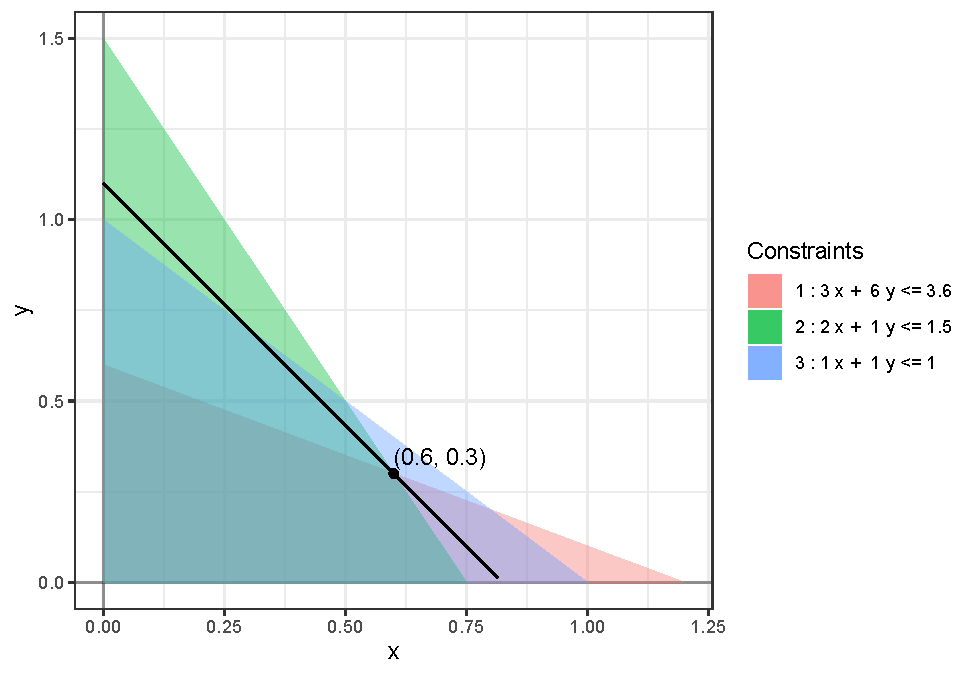
\includegraphics{Introduction-to-Optimization_files/figure-latex/fig-bond-portfolio-1.pdf}

The feasible set is the quadrilateral formed by the overlap of all three constraint regions. The level sets of the objective function are straight lines of the form \(4x + 3y = c\). We can see that the largest value of \(c\) for which these level sets intersect the feasible region turns out to be \(c = 3.3\%\) for \((x, y) = (0.6, 0.3)\).

\begin{exercise}
What are some possible ways to relax the constraints in the above problem so that all the money can be invested? What is the improved annual yield?
\end{exercise}

\begin{exercise}

The following exercises review some basic facts about inequalities:

\begin{enumerate}
\def\labelenumi{\arabic{enumi}.}
\tightlist
\item
  Find constants \(a, b, c, d\) such that \(a < b\), \(c < d\), \(a - c < b - d\), and \(ac < bd\).
\item
  Find constants \(a, b, c, d\) such that \(a < b\), \(c < d\), \(a - c < b - d\), and \(ac > bd\).
\item
  Find constants \(a, b, c, d\) such that \(a < b\), \(c < d\), \(a - c > b - d\), and \(ac < bd\).
\item
  Find constants \(a, b, c, d\) such that \(a < b\), \(c < d\), \(a - c > b - d\), and \(ac > bd\).
\item
  Prove that if \(a, b, c, d\) are constants such that \(a < b\) and \(c < d\), then \(a + c < b + d\). Why does this proof fail when we try to subtract the two inequalities instead of adding them?
\end{enumerate}

\end{exercise}

\hypertarget{part-simplex-method}{%
\part{Simplex Method}\label{part-simplex-method}}

\hypertarget{standard-linear-program}{%
\chapter{Standard Linear Program}\label{standard-linear-program}}

Our first goal is to find a general method for solving linear programs.
However, instead of solving linear programs in their full generality, we'll construct an algorithm for solving standard linear programs.
We will see later that every linear program can be \emph{standardized} and hence it suffices to construct an algorithm for solving standard linear programs.

\begin{definition}
A \textbf{standard linear program} is an optimization problem of the following form:
\begin{equation}
  \begin{array}{lrrrrrrrrr}
    \mbox{maximize: } & c_0 & + & c_1 x_1 & + & \dots & + & c_n x_n & \\
    \mbox{subject to: } 
      & & & a_{11} x_1 & + & \dots & + & a_{1n} x_n & \leq & b_1 \\
      & & & a_{21} x_1 & + & \dots & + & a_{2n} x_n & \leq & b_2 \\
      & & & & & \vdots &  \\
      & & & a_{m1} x_1 & + & \dots & + & a_{mn} x_n & \leq & b_m \\
      & & & x_1, & x_2, & \dots &, & x_n & \geq & 0
  \end{array} 
  \label{eq:standard-lp}
\end{equation}
where \(c_i\), \(a_{ij}\), and \(b_j\) are real constants. The variables \(x_1, \dots, x_n\) are called \textbf{decision variables}. A tuple \((x_1, \dots, x_n)\) that satisfy \emph{all} the constraints is called a \textbf{feasible solution} and the set of all feasible solutions is called the \textbf{feasible region}.
\end{definition}

\begin{example}
Equation \eqref{eq:bond-portfolio-lp} is an example of a standard linear program with 2 decision variables, 3 constraints, and the feasible region being a quadrilateral.
\end{example}

\begin{definition}
For each constraint, we introduce a \textbf{slack variable} by subtracting the LHS from the RHS as follows.
\begin{equation}
  \begin{array}{lrrrrrrrrr}
      w_1 & = & b_1 & - & a_{11} x_1 & - & \dots & - & a_{1n} x_n \\
      w_2 & = & b_2 & - & a_{21} x_1 & - & \dots & - & a_{2n} x_n \\
      & & & & & \vdots &  \\
      w_m & = & b_m & - & a_{m1} x_1 & - & \dots & - & a_{mn} x_n 
  \end{array} 
  \label{eq:slack-variables-def}
\end{equation}
\end{definition}

We can think of the slack variable \(w_i\) as measuring the \emph{slackness} in the \(i^{th}\) constraint. The \(i^{th}\) constraint is strictly met exactly when \(w_i\) is zero. Using the slack variables, the linear program \eqref{eq:standard-lp} can be succinctly rewritten as:
\begin{equation*}
  w_1, \dots, w_m, x_1, \dots, x_n \geq 0.
\end{equation*}

\begin{example}
The slack variables for the linear program \eqref{eq:bond-portfolio-lp} are as follows:
\begin{equation*}
  \begin{array}{rlllllll}
  w_1 & = & 3.6 & - & 3x & - & 6y \\
  w_2 & = & 1.5 & - & 2x & - & y \\
  w_3 & = & 1 & - & x & - & y.
  \end{array}
\end{equation*}
In terms of these slack variables, the constraints can be rewritten as \(x, y, w_1, w_2, w_3 \ge 0\) and the boundaries of the feasible region are given by \(x = 0, y = 0, w_1 = 0, w_2 = 0, w_3 = 0\).

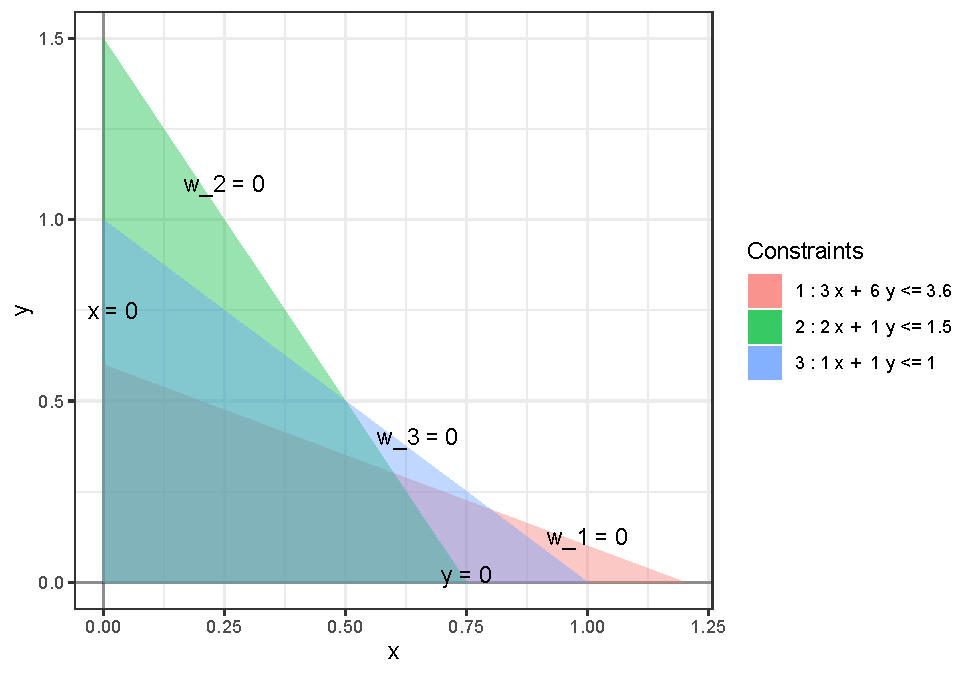
\includegraphics{Introduction-to-Optimization_files/figure-latex/fig-bond-portfolio-slack-1.pdf}
\end{example}

To construct the simplex method, we need a few facts about the geometry of the feasible region.

\begin{definition}
\protect\hypertarget{def:degeneracy}{}\label{def:degeneracy}A \textbf{basic feasible solution} of the standard linear program \eqref{eq:standard-lp} is defined as a feasible solution at which at least \(n\) basic or decision variables equal 0. A BFS where exactly \(n\) basic or decision variables are 0 is called \textbf{non-degenerate}. A BFS where more than \(n\) basic or decision variables are 0 is called \textbf{degenerate}. At a non-degenerate BFS, the \(n\) variables that equal 0 are called \textbf{non-basic} and the remaining \(m\) variables are called \textbf{basic}.
At a degenerate BFS, we choose some \(n\) vanishing variables to be non-basic and call the rest of the variables basic.
\end{definition}

\begin{example}
The feasible region for the linear program \eqref{eq:bond-portfolio-lp} has four non-degenerate basic feasible solutions: \((0,0)\), \((0.75, 0)\), \((0, 0.6)\), and \((0.6, 0.3)\) and the optimal solution is attained at the BFS \((0.6, 0.3)\). At the origin, the non-basic variables are \(x, y\) and the basic variables are \(w_1, w_2, w_3\). At the optimal solution, the non-basic variables are \(w_1, w_2\) and the basic variables are \(x, y, w_3\).
\end{example}

We will assume the following theorem without proof.

\begin{theorem}[Fundamental theorem of linear programming]

For a standard linear program, exactly on of the following holds:

\begin{enumerate}
\def\labelenumi{\arabic{enumi}.}
\tightlist
\item
  There is no feasible solution. In this case, we call the linear program \textbf{infeasible}.
\item
  The optimal value can grow arbitrary large on the feasible region. In this case, we call the linear program \textbf{unbounded}.
\item
  There is an optimal solution. In this case, we can further say that then there is a basic feasible solution which is optimal.
\end{enumerate}

\end{theorem}

The hardest step in the proof of the Fundamental theorem is showing that some basic feasible solution is optimal, if an optimal solution exists. One way to show this is by showing that the simplex method, which finds basic feasible solutions, always halts whenever an optimal solution exists. As we'll see in the following chapters, proving this is true in the case of degeneracies is beyond the scope of this class.

\hypertarget{the-simplex-method}{%
\chapter{The Simplex Method}\label{the-simplex-method}}

The simplex method is an iterative process for finding the optimal solution of a standard linear program. It starts at some BFS and in each step moves to an adjacent BFS with a higher objective value. The following picture shows one possible run of the simplex method for solving the linear program \eqref{eq:bond-portfolio-lp}.

\begin{figure}
\centering
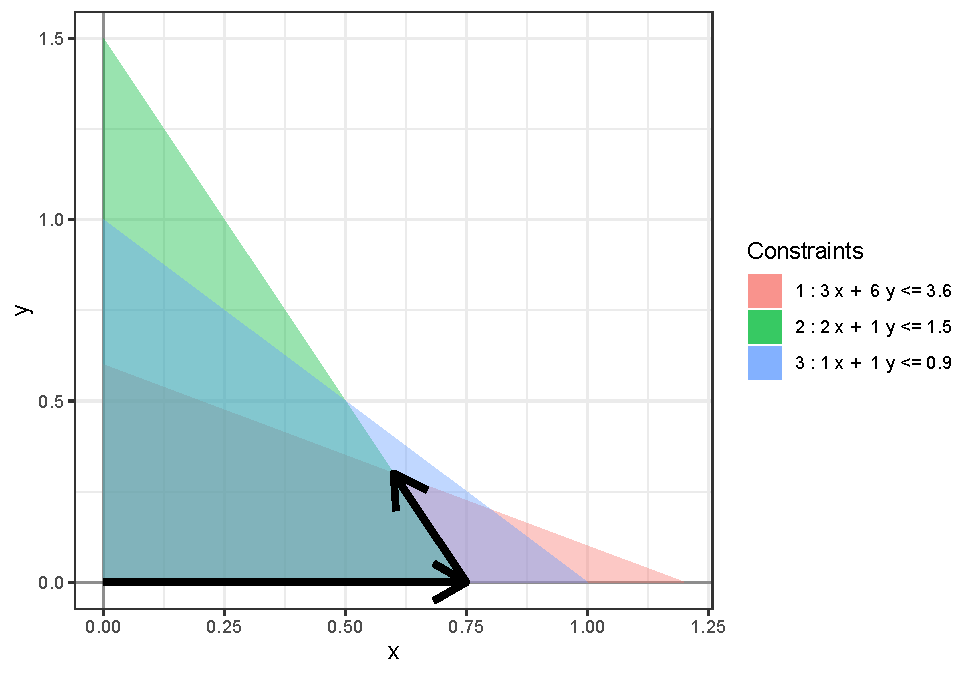
\includegraphics{Introduction-to-Optimization_files/figure-latex/sample-run-1.pdf}
\caption{\label{fig:sample-run}A possible run of the simplex algorithm.}
\end{figure}

In each step, one non-basic variable \textbf{enters} the set of basic variables and one basic variable \textbf{leaves} the set of basic variables. The table below explains how these sets are getting updated in the sample simplex algorithm run in Figure \ref{fig:sample-run}.

\begin{longtable}[]{@{}lllll@{}}
\toprule
& Leaving variable & Entering variable & Basic variables & Non-basic variables \\
\midrule
\endhead
Start & & & \(\{w_1, w_2, w_3\}\) & \(\{x, y\}\) \\
Step 1 & \(w_2\) & \(x\) & \(\{w_1, x, w_3\}\) & \(\{w_2, y\}\) \\
Step 2 & \(w_1\) & \(y\) & \(\{y, x, w_3\}\) & \(\{w_2, w_1\}\) \\
\bottomrule
\end{longtable}

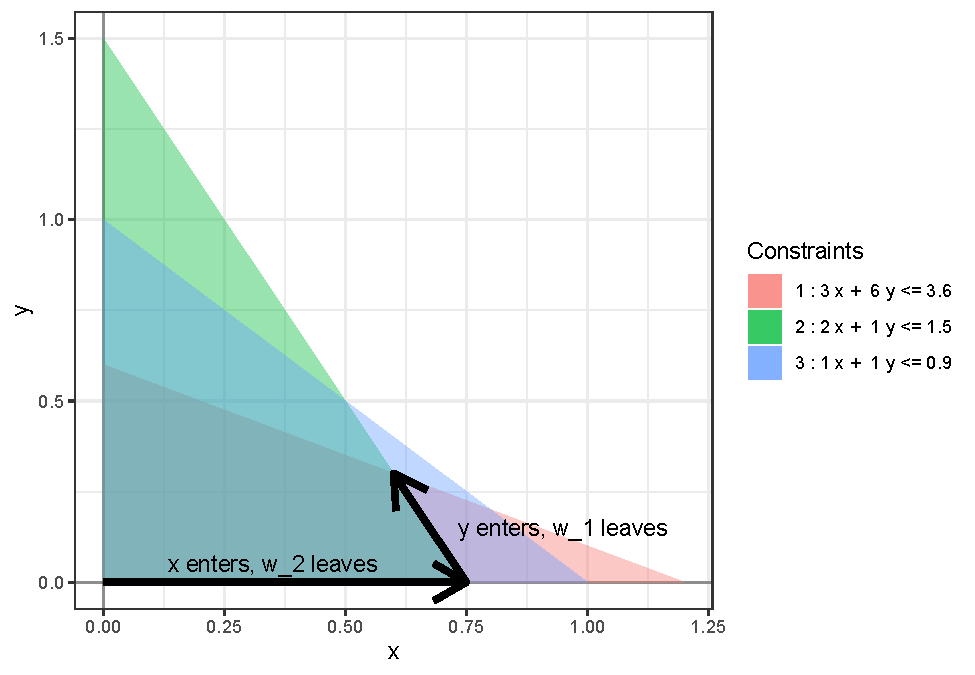
\includegraphics{Introduction-to-Optimization_files/figure-latex/fig-bond-portfolio-entering-1.pdf}

Using this terminology, our goal at each step is reduced to finding the entering and leaving variables.
To do this algebraically, we'll introduce the notion of dictionaries.

\begin{definition}
The \textbf{dictionary} at a basic feasible solution is a set of equations describing the objective function and the constraints in terms of the non-basic variables.
\end{definition}

\begin{example}
\protect\hypertarget{exm:dictionaries}{}\label{exm:dictionaries}Consider \eqref{eq:bond-portfolio-lp} again. At the origin, the non-basic variables are \(x, y\) and hence the initial dictionary is:
\begin{equation}
  \begin{array}{rlrrrrr}
  \mbox{objective} & = & 0 & + & 4x & + & 3y \\
  w_1 & = & 3.6 & - & 3x & - & 6y \\
  w_2 & = & 1.5 & - & 2x & - & y \\
  w_3 & = & 1 & - & x & - & y.
  \end{array}
  \label{eq:example-dictionary-1}
\end{equation}
After the first step of the simplex algorithm, the non-basic variables are \(w_2, y\). We can write \(x\) in terms of \(w_2\) to get
\begin{equation*}
  x = 0.75 - 0.5 w_2 - 0.5 y
\end{equation*}
We can substitute this into the initial dictionary to get the dictionary after the first step:
\begin{equation}
  \begin{array}{rlrrrrr}
  \mbox{objective} & = & 3 & + & (-2)w_2 & + & y \\
  w_1 & = & 1.35 & - & (-1.5) w_2 & - & 4.5y \\
  x & = & 0.75 & - & 0.5 w_2 & - & 0.5y \\
  w_3 & = & 0.25 & - & (-0.5) w_2 & - & 0.5y.
  \end{array}
  \label{eq:example-dictionary-2}
\end{equation}
Finally, the non-basic variables at the optimal solution are \(w_1, w_2\).
We can repeat the above process and get the dictionary for the optimal solution:
\begin{equation}
  \begin{array}{rlrrrrr}
  \mbox{objective} & = & 3.3 & + & (-5/3)w_2 & + & (-2/9)w_1 \\
  y & = & 0.3 & - & (-1/3) w_2 & - & 2/9 w_1 \\
  x & = & 0.6 & - & 2/3 w_2 & - & (-1/9) w_1 \\
  w_3 & = & 0.1 & - & (-1/3) w_2 & - & (-1/9) w_1.
  \end{array}
  \label{eq:example-dictionary-3}
\end{equation}
\end{example}

\begin{remark}
From the dictionary, one can extract the set of basic variables and the set of non-basic variables by looking at the variables appearing on the LHS and RHS, respectively. Furthermore, by setting the non-basic variables to 0, we obtain the very useful fact that

\begin{itemize}
\tightlist
\item
  the values of the basic variables are simply the constants ``\(b_i\)'', and
\item
  the value of the objective function is the constant ``\(c_0\)''.
\end{itemize}

For example, from the final dictionary above, we can immediately see that \(x = 0.6\), \(y = 0.3\), \(w_3 = 0.9\), and the objective value is \(3.3%
\) (and \(w_1 = 0\) and \(w_2 = 0.3\)) at the optimal solution.
\end{remark}

\hypertarget{the-simplex-step}{%
\section{The Simplex Step}\label{the-simplex-step}}

Suppose we are at a BFS. Let \(\bar{w}_1, \dots, \bar{w}_m\) be the basic variables, \(\bar{x}_1, \dots, \bar{x}_n\) be the non-basic variables. Let \(\bar{c}_j\), \(\bar{b}_i\), and \(\bar{a}_{ij}\) be the constants appearing in the dictionary at the BFS so that the dictionary is as follows:
\begin{equation}
  \begin{array}{rrrrrrrrrr}
  \mbox{objective} & = & \bar{c}_0 & + & \bar{c}_1\bar{x}_1 & + & \dots & + & \bar{c}_n\bar{x}_n \\
      \bar{w}_1 & = & \bar{b}_1 & - & \bar{a}_{11} \bar{x}_1 & - & \dots & - & \bar{a}_{1n} \bar{x}_n \\
      \bar{w}_2 & = & \bar{b}_2 & - & \bar{a}_{21} \bar{x}_1 & - & \dots & - & \bar{a}_{2n} \bar{x}_n \\
      & & & & & \vdots &  \\
      \bar{w}_m & = & \bar{b}_m & - & \bar{a}_{m1} \bar{x}_1 & - & \dots & - & \bar{a}_{mn} \bar{x}_n 
  \end{array} 
  \label{eq:standard-dictionary}
\end{equation}
The first step is to choose the \emph{direction of the simplex step}.
Algebraically, this is done by choosing the entering variable.
We want to move to an adjacent BFS with a higher objective value. The current objective function is
\begin{align*}
  \bar{c}_0  +  \bar{c}_1\bar{x}_1  +  \dots  +  \bar{c}_n\bar{x}_n.
\end{align*}
and the current objective value is \(\bar{c}_0\) as all the non-basic variables \(\bar{x}_j\) are equal 0.
We can move away from the current BFS by increasing one of the non-basic variables \(\bar{x}_j\) from 0 to a positive value. The objective value will increase if \(\bar{c}_j > 0\). This then is the criterion for choosing the entering variable.

\begin{proposition}[Entering variable]
\protect\hypertarget{prp:entering-variable}{}\label{prp:entering-variable}A non-basic variable \(\bar{x}_j\) can be entering if \(\bar{c}_j > 0\).
\end{proposition}

\begin{example}
In the dictionary \eqref{eq:example-dictionary-1}, the objective function is \(4x + 3y\). Hence, both \(x\) and \(y\) can be chosen as the entering variables. Geometrically, we can see that there are two different paths going from the origin to the optimal solution. In the dictionary \eqref{eq:example-dictionary-2}, the objective function is \(3 + (-2)w_2 + y\) and only \(y\) can be the entering variable. In dictionary \eqref{eq:example-dictionary-3}, the objective function is \(3.3 + (-5/3)w_2 + (-2/9)w_1\) and there cannot be any entering variable.
\end{example}

Suppose \(\bar{x}_j\) is the chosen entering variable.
This determines the direction of the simplex step.
We next need to figure out the amount by which to increase \(\bar{x}_j\) without leaving the feasible region.
The basic variables are related to \(\bar{x}_j\) by the following relations
\begin{align*}
  \bar{w}_i = \bar{b}_i - \bar{a}_{ij} \bar{x}_j - \sum \limits_{k = 1, k \neq j}^{n}  \bar{a}_{ik} \bar{x}_k.
\end{align*}
The summation quantity stays at 0.
As \(x_j\) increases \(w_i\) will decrease exactly when \(a_{ij} > 0\).
Because we want all the variables to be non-negative, we must always have \(w_i = b_i - a_{ij} x_j \ge 0\).
This condition must hold true for all such \(w_i\). Hence, we get the following criterion for choosing the leaving variable.

\begin{proposition}[Leaving variable]
\protect\hypertarget{prp:leaving-variable}{}\label{prp:leaving-variable}Suppose \(\bar{x}_j\) is the entering variable. A basic variable \(\bar{w}_i\) can be chosen to be the leaving variable if
\begin{align*}
  i = {\arg \min} _{a_{ij} > 0} \dfrac{b_i}{a_{ij}}.
\end{align*}
\end{proposition}

In this case, after the simplex step \(w_i\) decreases to \(0\), \(x_j\) increases to \(\min_{a_{ij} > 0} {b_i}/{a_{ij}}\), and the objective value increases by \(\bar{c}_j \min_{a_{ij} > 0} {b_i}/{a_{ij}}\).

\begin{example}

In the dictionary \eqref{eq:example-dictionary-1}, if we choose \(x\) to be our entering variable then we need to get the following ratios to compare

\begin{longtable}[]{@{}cccc@{}}
\toprule
\(i\) & \(\bar{a}_{ij}\) & \(\bar{b}_i\) & \(\bar{b}_i/\bar{a}_{ij}\) \\
\midrule
\endhead
1 & 3 & 3.6 & 1.2 \\
2 & 2 & 1.5 & 0.75 \\
3 & 1 & 1 & 1 \\
\bottomrule
\end{longtable}

\end{example}

We can see that the smallest ratio is obtained for \(w_2\). Hence, it is the only candidate for the leaving variable.

\hypertarget{tableau-notation}{%
\section{Tableau Notation}\label{tableau-notation}}

When manipulating linear systems, one can forget the variables and simply perform manipulations on the coefficients using matrices.
The same is true for linear programs.
We start by rewriting the constraints in the dictionary with all the variables on the LHS and all the constants on the RHS:
\begin{equation}
  \begin{array}{rrrrrrrrrrrrrr}
      \bar{a}_{11} \bar{x}_1 & + & \dots & + & \bar{a}_{1n} \bar{x}_n & + & \bar{w}_1 & & & & & & = &  \bar{b}_1\\
      \bar{a}_{21} \bar{x}_1 & + & \dots & + & \bar{a}_{2n} \bar{x}_n & & & + & \bar{w}_2 & & & & = &  \bar{b}_2\\
      & & & & & \vdots &  \\
      \bar{a}_{m1} \bar{x}_1 & + & \dots & + & \bar{a}_{mn} \bar{x}_n & & & & & & + & \bar{w}_m & = & \bar{b}_m\\
  \end{array} 
  \label{eq:standard-tableau}
\end{equation}
This can then be encoded using the following augmented matrix:
\begin{equation*}
  \begin{array}{rrrrrrrrrrr|r}
      \bar{a}_{11}  & & \dots & & \bar{a}_{1n}  & 1 & & & & & &\bar{b}_1\\
      \bar{a}_{21}  & & \dots & & \bar{a}_{2n}  & & & 1 & & & &\bar{b}_2\\
      & & & & & \vdots &  \\
      \bar{a}_{m1}  & & \dots & & \bar{a}_{mn}  & & & & & & 1 &\bar{b}_m\\
  \end{array}
\end{equation*}
We add back the objective function, but because of a quirk of algebra we need to add the objective function coefficients as follows.
\begin{equation*}
 \begin{array}{rrrrrrrrrrr|r}
      \bar{a}_{11}  & & \dots & & \bar{a}_{1n}  & 1 & & & & & &\bar{b}_1\\
      \bar{a}_{21}  & & \dots & & \bar{a}_{2n}  & & & 1 & & & &\bar{b}_2\\
      & & & & & \vdots &  \\
      \bar{a}_{m1}  & & \dots & & \bar{a}_{mn}  & & & & & & 1 &\bar{b}_m\\ \hline
      \bar{c}_1  & & \dots & & \bar{c}_{n}  & 0 & & 0 & \dots & & 0 &-\bar{c}_0
  \end{array} 
\end{equation*}
The columns in this augmented matrix correspond to the variables \(\bar{x}_j\) and \(\bar{w}_i\). The columns with the \emph{pivots} correspond to the basic variables.

If \(\bar{x}_j\) is the entering variable and \(\bar{w}_i\) is the leaving variable, then we simply perform elementary row operations and turn the entry \(\bar{a}_{ij}\) into a pivot for its column. Hence, this step is also called the \textbf{pivot step}.

\begin{example}
The tableau corresponding to the dictionary \eqref{eq:example-dictionary-1} is as follows:
\begin{equation*}
  \begin{array}{lllll|l}
    3 & 6 & 1 & 0 & 0 & 3.6 \\
    \boxed{2} & 1 & 0 & 1 & 0 & 1.5 \\
    1  & 1 & 0 & 0 & 1 & 1 \\ \hline 
    4 & 3 & 0 & 0 & 0 & 0
  \end{array}
\end{equation*}
If we choose \(x\) as the entering variable and \(w_2\) as the leaving variable then we need to pivot about the entry \(a_{21}\) using elementary row operations to get the following tableau:
\begin{equation*}
  \begin{array}{lllll|l}
    0 & 4.5 & 1 & -1.5 & 0 & 1.35 \\
    \boxed{1} & 0.5 & 0 & 0.5 & 0 & 0.75 \\
    0  & 0.5 & 0 & -0.5 & 1 & 0.25 \\ \hline
    0 & 1 & 0 & -2 & 0 & -3
  \end{array}
\end{equation*}
which corresponds to the dictionary \eqref{eq:example-dictionary-2}.
\end{example}

\hypertarget{initialization}{%
\chapter{Initialization}\label{initialization}}

We now know how to move from a BFS to an adjacent one with a higher objective value.
We can start the simplex method at the origin if the origin is a BFS. However, this is not always the case.

\begin{proposition}
The origin is a basic feasible solution of the standard linear program \eqref{eq:standard-lp} if and only if \(b_i \ge 0\) for all \(1 \le i \le m.\)
\end{proposition}

When the origin is not a BFS, we need a process to find some vertex of the feasible region.
This is called the \textbf{Initialization Phase} or \textbf{Phase I} of the simplex method.
To do this we need to create an auxiliary linear program.

\hypertarget{auxiliary-linear-program}{%
\section{Auxiliary Linear Program}\label{auxiliary-linear-program}}

\begin{definition}
We say that a linear program is \textbf{feasible} if its feasible region is non-empty.
\end{definition}

The initialization phase determines if a standard linear program is feasible and if it is then it finds a BFS by solving the following auxiliary linear program.

\begin{definition}
The \textbf{auxiliary linear program} of the standard linear program \eqref{eq:standard-lp} is defined as follows:
\begin{equation}
  \begin{array}{lrrrrrrrrrrr}
    \mbox{maximize: } &  &  &   &  & &  & & - & x_0 & \\
    \mbox{subject to: } 
      & & & a_{11} x_1 & + & \dots & + & a_{1n} x_n & - &x_0 & \leq & b_1 \\
      & & & a_{21} x_1 & + & \dots & + & a_{2n} x_n & - &x_0 & \leq & b_2 \\
      & & & & & \vdots &  \\
      & & & a_{m1} x_1 & + & \dots & + & a_{mn} x_n & - &x_0 & \leq & b_m \\
      & & & x_1, & x_2, & \dots &, & x_n & , & x_0 & \geq & 0
  \end{array} 
  \label{eq:auxiliary-lp}
\end{equation}
\end{definition}

To understand the auxiliary linear program, it is better to write it in the following non-standard form:
\begin{equation*}
  \begin{array}{lrrrrrrrrrrrrr}
    \mbox{minimize: } & & & & & & & & & & & x_0 & \\
    \mbox{subject to: } 
      & & & a_{11} x_1 & + & \dots & + & a_{1n} x_n & \leq & b_1 & + & x_0 \\
      & & & a_{21} x_1 & + & \dots & + & a_{2n} x_n & \leq & b_2 & + & x_0 \\
      & & & & & \vdots &  \\
      & & & a_{m1} x_1 & + & \dots & + & a_{mn} x_n & \leq & b_m & + & x_0 \\
      & & & x_1, & x_2, & \dots &, & x_n & , & x_0 & \geq & 0
  \end{array} 
\end{equation*}
We can interpret \(x_0\) as a relaxation of the constraints. The auxiliary linear program is then asking - \emph{what is the smallest constraint relaxation necessary to make our linear program feasible?}. The primary linear program should feasible if and only if no relaxation is necessary. This is indeed the case.

\begin{exercise}
Show that the auxiliary linear program \eqref{eq:auxiliary-lp} is always feasible by explicitly constructing a feasible solution.
\end{exercise}

\begin{exercise}
Show that the objective values of the auxiliary linear program \eqref{eq:auxiliary-lp} are bounded from above by 0. Using the \href{https://en.wikipedia.org/wiki/Extreme_value_theorem}{extreme value theorem}, conclude that \eqref{eq:auxiliary-lp} always has an optimal solution.
\end{exercise}

Finally, we get the following theorem (proof left as an exercise) which provides an explicit connection between the optimal solution of the auxiliary linear program and the feasible region of the standard linear program

\begin{theorem}
\protect\hypertarget{thm:auxiliary-lp}{}\label{thm:auxiliary-lp}Suppose \((k_1, k_2, \dots, k_n, k_0)\) is an optimal solution of the auxiliary linear program \eqref{eq:auxiliary-lp}. Then, the standard linear program \eqref{eq:standard-lp} is feasible if and only if \(k_0 = 0\). In this case, \((k_1, k_2, \dots, k_n)\) is a basic feasible solution of \eqref{eq:standard-lp}.
\end{theorem}

So, our problem is not reduced to determining the optimal solution of the auxiliary linear program.
Note that the origin is not in the feasible region, so we cannot start applying the simplex steps.
The following exercise provides us a way to find a BFS of the auxiliary linear program.

\begin{exercise}
Suppose some \(b_i\) is negative.
Without any loss of generality, assume that \(b_1\) is the smallest among all the \(b_i\) (i.e.~the most negative).
Show that after the pivot step in tableau about the column corresponding to \(x_0\) and the row corresponding to \(w_1\), all the \(b_i\)'s become positive.
\end{exercise}

To summarize, if the origin is not a vertex of the feasible region, then the method of solving the standard linear program \eqref{eq:standard-lp}, starting with \textbf{Phase I}, is as follows:

\begin{enumerate}
\def\labelenumi{\arabic{enumi}.}
\tightlist
\item
  Form the auxiliary linear program and its tableau.
\item
  Perform a pivot operation about the entry in the column corresponding to the variable \(x_0\) and the row corresponding to the \emph{most negative \(b_i\)}. This results in a dictionary where all the \(b_i\)'s are now non-negative.
\item
  Solve the auxiliary linear program by repeatedly performing pivot steps.
  Suppose \((k_1, k_2, \dots, k_n, k_0)\) is an optimal solution of the auxiliary linear program.

  \begin{enumerate}
  \def\labelenumii{\arabic{enumii}.}
  \tightlist
  \item
    If \(k_0 \neq 0\), then we halt as the primary linear program is not feasible.
  \item
    If \(k_0 = 0\), then we proceed to \textbf{Phase II}. We start solving the original linear program starting at the BFS \((k_1, \dots, k_n)\) by repeatedly performing pivot steps.
  \end{enumerate}
\end{enumerate}

\hypertarget{combined-tableau}{%
\section{Combined tableau}\label{combined-tableau}}

In the above algorithm, at the end of Phase I, we need to calculate the dictionary at the \$BFS \((k_1, \dots, k_n)\) when starting Phase II. We can avoid this recalculation by instead manipulating a \emph{combined tableau} which contains information about both the auxiliary linear program and the primary linear program.

\begin{definition}
The combined tableau is defined as follows:
\begin{equation*}
  \begin{array}{rrrrrrrrrrrr|l}
      a_{11}  & & \dots & & a_{1n}  & 1 & & & & & & -1 &b_1\\
      a_{21}  & & \dots & & a_{2n}  & & & 1 & & & & -1 &b_2\\
      & & & & & \vdots & & & & & & \vdots & \vdots \\
      a_{m1}  & & \dots & & a_{mn}  & & & & & & 1 & -1 &b_m\\ \hline
      c_1  & & \dots & & c_{n}  & 0 & & 0 & \dots & & 0 & 0 & 0\\ \hline
      0  & & \dots & & 0  & 0 & & 0 & \dots & & 0 & -1 & 0
  \end{array} 
\end{equation*}
\end{definition}

The second last row of the tableau corresponds to the objective function of the primary linear program and the last row of the tableau corresponds to the objective of the auxiliary linear program. We use the combined tableau to first perform Phase I and then neglect the auxiliary objective and the variable \(x_0\) and proceed on to Phase II using the same tableau.

\begin{example}
Consider the following linear program:
\begin{equation*}
  \begin{array}{rrrrrl}
  \mbox{maximize:} & x & + & y \\
  \mbox{subject to:}
    & x & + & 2y & \le & 6 \\
    & -x &  &  & \le & -1 \\ 
    &  &  & -y & \le & -2 \\ 
    & x & , & y & \ge & 0.
  \end{array}
\end{equation*}
Because \((0,0)\) is not feasible, we need to start with the initialization phase. We form the combined tableau:
\begin{equation*}
  \begin{array}{rrrrrr|r}
    1 & 2 & 1 & 0 & 0 & -1 & 6 \\
    -1 & 0 & 0 & 1 & 0 & -1 & -1 \\
    0 & -1 & 0 & 0 & 1 & \boxed{-1} & -2 \\ \hline
    1 & 1 & 0 & 0 & 0 & 0 & 0 \\ \hline
    0 & 0 & 0 & 0 & 0 & -1 & 0 
  \end{array}
\end{equation*}
The first pivot is in the column corresponding to the variable \(x_0\) and the row corresponding to the \emph{most negative \(b_i\)} (which is \(b_3 = -2\)). This results in the following combined tableau:
\begin{equation*}
  \begin{array}{rrrrrr|r}
    1 & 3 & 1 & 0 & -1 & 0 & 8 \\
    -1 & 1 & 0 & 1 & -1 & 0 & 1 \\
    0 & 1 & 0 & 0 & -1 & 1 & 2 \\ \hline
    1 & 1 & 0 & 0 & 0 & 0 & 0 \\ \hline
    0 & 1 & 0 & 0 & -1 & 0 & 2 
  \end{array}
\end{equation*}
We then continue performing pivot steps to find the solution:
\begin{equation*}
  \begin{array}{rrrrrr|r}
    0 & 0 & 1 & 1 & 2 & -4 & 1 \\
    0 & 1 & 0 & 0 & -1 & 1 & 2 \\
    1 & 0 & 0 & -1 & 0 & 1 & 1 \\ \hline
    0 & 0 & 0 & 1 & 1 & -2 & -3 \\ \hline
    0 & 0 & 0 & 0 & 0 & -1 & \mathbf{0} 
  \end{array}
\end{equation*}
We see that the optimal value is 0 and hence the primary linear program is feasible. We then remove the auxiliary objective and coefficient to get the following tableau for the primary linear program:
\begin{equation*}
  \begin{array}{rrrrr|r}
    0 & 0 & 1 & \boxed{1} & 2  & 1 \\
    0 & 1 & 0 & 0 & -1 & 2 \\
    1 & 0 & 0 & -1 & 0 & 1 \\ \hline
    0 & 0 & 0 & 1 & 1  & -3
  \end{array}
\end{equation*}
Continuing with the simplex method we get the following final tableau
\begin{equation*}
  \begin{array}{rrrrr|r}
    0 & 0 & 1 & 1 & 2 & 1 \\
    0 & 1 & 0 & 0 & -1 & 2 \\
    1 & 0 & 1 & 0 & 2 & 2 \\ \hline
    0 & 0 & -1 & 0 & -1 & -4 
  \end{array}
\end{equation*}
The final non-basic variables are \(w_1\) and \(w_3\), the basic variables are \(x\), \(y\), \(w_2\) with values \(2\), \(2\), \(1\), respectively, and the optimal objective value is \(4\).
\end{example}

\hypertarget{cycling}{%
\chapter{Cycling}\label{cycling}}

We know how to start the simplex method and how to perform the pivot steps.
We'll next analyze the halting conditions for the simplex method.
We will not be able to perform the pivot steps if no entering or leaving variables are found.

If no entering variable is found, then the geometry tells us that there is no direction in which the objective value can be increased i.e.~we're at a local maxima.
But because the objective function is a linear function this local maxima is also an absolute maxima and \textbf{provides an optimal solution to our linear program}. Algebraically, this happens when none of the \(\bar{c}_i\) are positive.

\begin{proposition}
If none of the objective coefficients \(\bar{c}_i\) are positive in the current dictionary, then the current BFS is optimal.
\end{proposition}

If no leaving variable is found, then the geometry tells us that we can keep increasing the entering variable indefinitely without leaving the feasible region. Such a linear program is called \textbf{unbounded}.
An unbounded linear program has no optimal solution as the objective value can be made arbitrary large without leaving the feasible region. Algebraically, this happens when none of the \(\bar{a}_{ij}\) are positive.

\begin{proposition}
Suppose \(\bar{x}_j\) is the entering variable. If none of the constants \(\bar{a}_{ij}\) are positive in the current dictionary, then the linear program is unbounded.
\end{proposition}

Another point of failure is in the initialization phase. We've already seen that if the initialization phase fails then there is no feasible solution. We restate the result here for completion.

\begin{proposition}
If some \(b_i\) is negative, and the initialization phase fails then the linear program is infeasible.
\end{proposition}

Unfortunately, the above results are not sufficient to guarantee that the simplex method will always find a solution if one exists. It is possible for the simplex method to get stuck in a loop. This is called \textbf{cycling}.

\begin{exercise}
Give an example showing that the variable that enters in one pivot step can become leave in the next.
\end{exercise}

\begin{exercise}
Show that the variable that leaves in one pivot step cannot enter in the next.
\end{exercise}

\hypertarget{degeneracy}{%
\section{Degeneracy}\label{degeneracy}}

Cycling does not always occur when running the simplex method. We saw in Section \ref{the-simplex-step} that after the pivot step the entering and leaving variable gets updated as follows:
\begin{align*}
  \bar{x}_j & \mapsto \bar{b}_i/\bar{a}_{ij} \\
  \bar{w}_i & \mapsto 0.
\end{align*}
This increases the value of the objective function by \(\bar{c}_j \bar{b}_i/\bar{a}_{ij}\).
Because of the criterion for choosing the entering and leaving variables, the constants \(\bar{c}_i\) and \(\bar{a}_{ij}\) are always positive. We know that \(\bar{b}_i\) this is the value of the basic variable \(\bar{w}_i\) and hence must be greater than or equal to 0.
If \(\bar{b}_i > 0\) then the objective value will increase in the pivot step and we will never return back to this BFS.
Hence, the only case when cycling \emph{can} occur is when \(\bar{b}_i = 0\).
But \(\bar{b}_i\) is the value of the basic variable \(\bar{w}_i\).
Having more than \(n\) variables vanishing at a BFS is precisely the definition of degeneracy \ref{def:degeneracy}.

\begin{proposition}
The simplex method can cycle if there some degenerate BFS.
\end{proposition}

\begin{example}
The following slight modification of Example \eqref{eq:bond-portfolio-lp} is a degenerate linear program:
\begin{equation*}
  \begin{array}{rrrrrl}
  \mbox{maximize:} & 4x & + & 3y \\
  \mbox{subject to:}
    & 3x & + & 6y & \le & 4.5 \\
    & 2x & + & y & \le & 1.5 \\
    & x & + & y & \le & 1 \\
    & x & , & y & \ge & 0.
  \end{array}
\end{equation*}

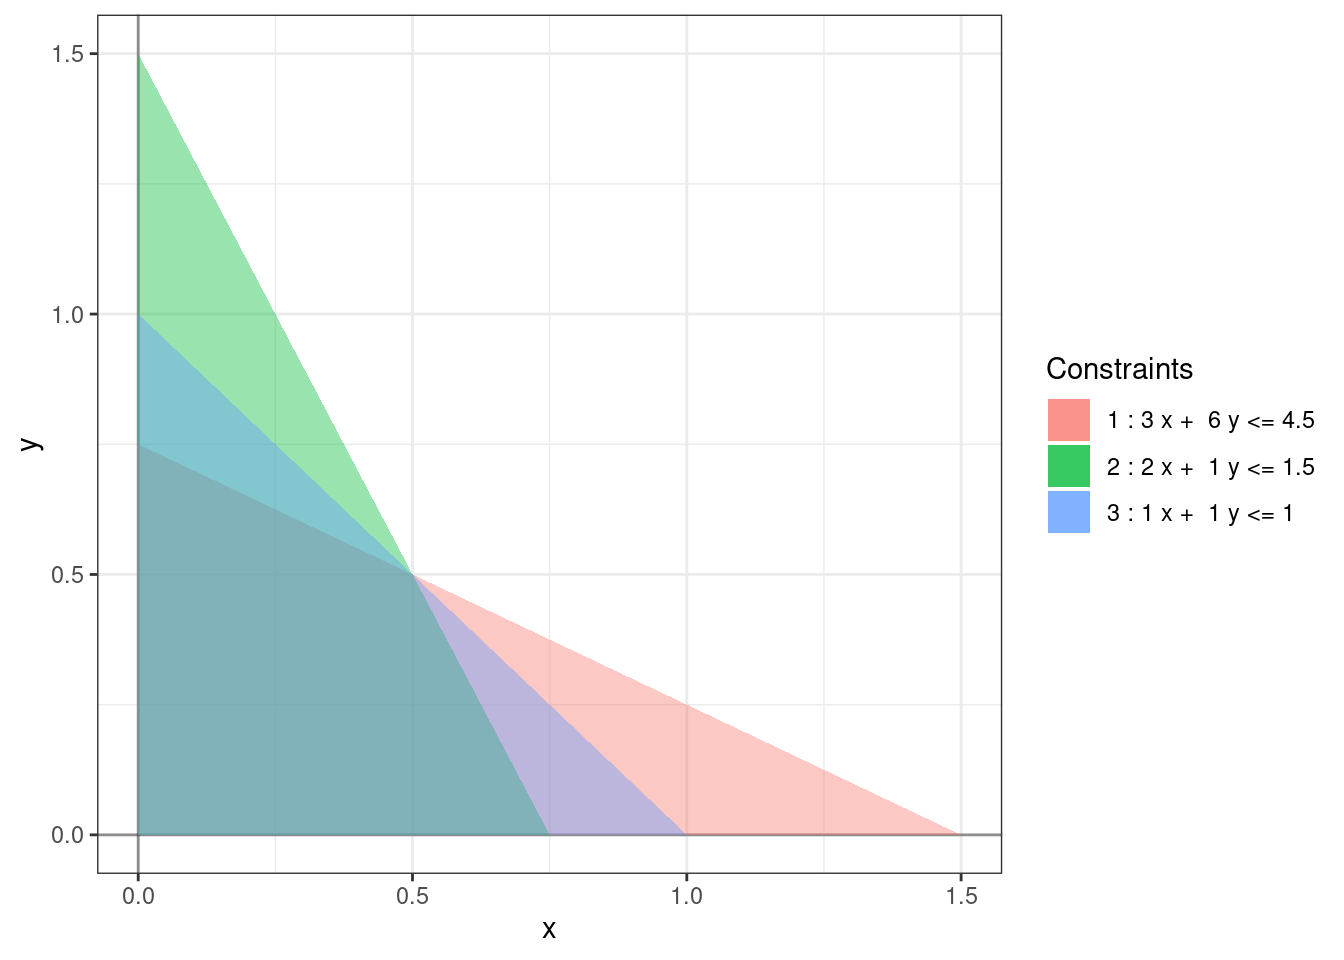
\includegraphics{Introduction-to-Optimization_files/figure-latex/fig-degenerate-lp-1.pdf}

At the optimal solution, \((0.5, 0.5)\) all three constraints are met. At this BFS, one of the rows is
\begin{align}
  w_3 &= 0 + 0.33 w_2 + 0.11 w_1.
\end{align}
\end{example}

\begin{example}
\protect\hypertarget{exm:cycling}{}\label{exm:cycling}Consider the following degenerate linear program:
\begin{equation*}
  \begin{array}{rrrrrrrrrl}
  \mbox{maximize:} & x_1 & - & 2x_2 & & & - & 2x_4 \\
  \mbox{subject to:}
    & 0.5 x_1 & - & 3.5x_2 & - & 2x_3 & + & 4 x_4 & \le & 0 \\
    & 0.5 x_1 & - & x_2 & - & 0.5 x_3 & + & 0.5 x_4 & \le & 0 \\
    & x_1 & & & & &  &  & \le & 1 \\
    & x_1 & , & x_2 & , & x_3 & , & x_4 & \ge & 0 \\
  \end{array}
\end{equation*}
The following is a valid sequence of simplex steps:

\begin{enumerate}
\def\labelenumi{\arabic{enumi}.}
\tightlist
\item
  \(x_1\) enters and \(w_1\) leaves,
\item
  \(x_2\) enters and \(w_2\) leaves,
\item
  \(x_3\) enters and \(x_1\) leaves,
\item
  \(x_4\) enters and \(x_2\) leaves,
\item
  \(w_1\) enters and \(x_3\) leaves,
\item
  \(w_2\) enters and \(x_4\) leaves.
\end{enumerate}

At the end of the \(6^{th}\) simplex step, we end up looping back to the origin.
\end{example}

\hypertarget{blands-rule}{%
\section{Bland's Rule}\label{blands-rule}}

There are various ways of dealing with cycling.
The simplest such way is called Bland's rule.
\textbf{Bland's rule} says that if there are multiple candidates for the entering/variable then we choose the one with the smallest index. (We assume that the decision variables have a smaller index than the slack variables.)

\begin{theorem}[Bland's rule]
The simplex method always terminates provided that both the
entering and the leaving variable are chosen according to Bland's rule.
\end{theorem}

The proof of this theorem is too complicated for this course. With this modification, for both Phase I and Phase II of the simplex method, we now have a complete algorithm for solving linear programs.

\begin{example}
In Example \ref{exm:cycling}, the \emph{sixth simplex step} violates Bland's rule. Both \(x_1\) and \(x_4\) can be leaving variables and we choose \(x_4\) whereas Bland's rule requires us to choose \(x_1\).
\end{example}

\hypertarget{standardization}{%
\chapter{Standardization}\label{standardization}}

We have an algorithm for solving a standard linear program.
We'll not extend it to more general linear programs, which is simply an optimization problem where the objective function is a linear program and the constraints are linear equalities or inequalities.

\begin{definition}
A \textbf{general linear program} is an optimization problem of the following form:
\begin{equation}
  \begin{array}{llllllll}
    \mbox{optimize: } 
      & c_1 x_1 & + & \dots & + & c_n x_n & \\
    \mbox{subject to: } 
      & a_{11} x_1 & + & \dots & + & a_{1n} x_n & \lesseqqgtr & b_1 \\
      & a_{21} x_1 & + & \dots & + & a_{2n} x_n & \lesseqqgtr & b_2 \\
      & & & \vdots &  \\
      & a_{m1} x_1 & + & \dots & + & a_{mn} x_n & \lesseqqgtr b_m,
  \end{array}
  \label{eq:intro-lp}
\end{equation}
where the symbol \(\lesseqqgtr\) stands for \(\leq\) or \(=\) or \(\geq\), \(a_{ij}, b_i, c_j\) are real numbers, and \(x_j\) are variables.
\end{definition}

We do not allow strict inequalities \(<\) or \(>\) in a linear program as linear functions do not always achieve maxima/minima on open sets even when the sets are bounded. Consider the following simple example.
\begin{align*}
  \mbox{maximize:} && x \\
  \mbox{subject to:} 
  && x &< 1 \\
  && x &\ge 0
\end{align*}
On the feasible set \([0, 1)\), the function \(x\) never attains absolute maxima.
Changing the inequality \(<\) to \(\leq\) gives us an optimal feasible solution \(x = 1\).

\hypertarget{equivalence-of-linear-programs}{%
\section{Equivalence of Linear Programs}\label{equivalence-of-linear-programs}}

Any linear program can be changed to a \emph{maximization problem} as minimizing a function is the same as maximizing its negation. From now on, we'll assume that the goal of our linear programs is to \emph{maximize} the objective function.

\begin{definition}
Two (maximizing) linear programs LP and LP' are said to be \textbf{equivalent} if for any feasible solution \((x_1, \dots, x_n)\) to LP, there exists a feasible solution \((x'_1, \dots, x'_{n'})\) to LP' with the same objective value and for any feasible solution \((y'_1, \dots, y'_n)\) to LP', there exists a feasible solution \((y_1, \dots, y_{n})\) to LP with the same objective value . Thus solving LP is equivalent to LP'.
\end{definition}

\begin{remark}
~
1. LP and LP' can have a different number of decision variables i.e.~we do not require \(n = n'.\)
2. There need not be a one-to-one correspondence between the feasible sets of LP and LP' i.e.~for a feasible solution to LP there could be multiple feasible solutions with the same objective value. Similarly, in the other direction.
\end{remark}

\begin{remark}
Even though equivalence of linear programs only requires the existence of an abstract correspondence between the feasible sets of LP and LP', in practice, one constructs linear transformations \(T: \mathbb{R}^n \to \mathbb{R}^{n'}\) and \(S: \mathbb{R}^{n'} \to \mathbb{R}^{n}\) which map the feasible set of LP to LP' and the feasible set of LP' to LP, respectively. These linear transformations need not be inverses of each other, or even isomorphisms. They only need to preserve the objective values.
\end{remark}

\begin{example}
The following two linear programs are equivalent to each other
\begin{align*}
\begin{aligned}
  \mbox{maximize: } && x + y & \\
  \mbox{subject to: } && 0 \le x &\le 1 \\
     && 0 \le y &\le 1 
\end{aligned}
&&
\begin{aligned}
  \mbox{maximize: } && z & \\
  \mbox{subject to: } && 0 \le z &\le 1
\end{aligned}
\end{align*}
via the transformations \(T(x, y) = x + y\) and \(S(z) = (z/2, z/2)\).
\end{example}

\begin{theorem}
\protect\hypertarget{thm:lp-to-standard-form}{}\label{thm:lp-to-standard-form}Every linear program is equivalent to a linear program in the standard form.
\end{theorem}

\begin{proof}

The proof is by providing an explicit \emph{standardization} algorithm. Consider the linear program in \eqref{eq:intro-lp}, where we're assuming that the goal is to maximize the objective function. If it is in the standard form, then we're done. If not, then there must be a finite number of \emph{errors} of the following types:

\begin{enumerate}
\def\labelenumi{\arabic{enumi}.}
\tightlist
\item
  A linear constraint is a lower bound and has the form \[a_{i1} x_1 + \dots + a_{in} x_n \geq b_i.\]
\item
  A linear constraint is an equality and has the form \[a_{i1} x_1 + \dots + a_{in} x_n = b_i.\]
\item
  A variable \(x_j\) has a \emph{negativity constraint} \(x_j \leq 0\).
\item
  A variable \(x_j\) is \textbf{free} i.e.~it is missing a \emph{sign constraint}.
\end{enumerate}

We fix these errors one at a time, while making sure that no new errors are introduced, thereby guaranteeing termination of the algorithm.

\begin{enumerate}
\def\labelenumi{\arabic{enumi}.}
\tightlist
\item
  We replace the constraint with \[ -a_{i1} x_1 + \dots + -a_{in} x_n \leq -b_i. \]
\item
  We replace the constraint with two constraints
  \begin{align*}
    a_{i1} x_1 + \dots + a_{in} x_n &\leq b_i \\
    -a_{i1} x_1 - \dots - a_{in} x_n &\leq -b_i,
    \end{align*}
\item
  We let \(y_j = -x_j\) and create a new linear program using the variables \(x_1\), \(\dots\), \(x_{j-1}\), \(y_j\), \(x_{j+1}\), \(\dots\), \(x_n\) by replacing \(x_j\) with \(-y_j\) everywhere.
\item
  We let \(x_j = y_j - z_j\) for two new decision variables \(y_j\) and \(z_j\) with \(y_j, z_j \geq 0\) and create a new linear program using the variables \(x_1\), \(\dots\), \(x_{j-1}\), \(y_j\), \(z_j\), \(x_{j+1}\), \(\dots\), \(x_n\) by replacing \(x_j\) with \(y_j - z_j\) everywhere. We can do this because any real number can written as a difference of two positive real numbers.
\end{enumerate}

\end{proof}

\begin{exercise}
\protect\hypertarget{exr:lp-to-standard-form}{}\label{exr:lp-to-standard-form}Prove that the algorithm in the proof of Theorem \ref{thm:lp-to-standard-form} produces a linear program that is equivalent to the original linear program.
\end{exercise}

\hypertarget{part-duality-theory}{%
\part{Duality Theory}\label{part-duality-theory}}

\hypertarget{dual-linear-program}{%
\chapter{Dual Linear Program}\label{dual-linear-program}}

So far we've constructed a method for solving linear programs.
Our next goal is to understand the dependence of the solution on the various constants in the program.
We will do this using duality theory.

We start by introducing the matrix notation. We'll let \(x\) denote the vector of decision variables, \(b\) the vector of upper bounds, \(c\) the vector of objective coefficients, and \(A\) the matrix of constraints in the standard linear program \eqref{eq:standard-lp}.
\begin{align*}
  x = \begin{bmatrix} x_1 \\ x_2 \\ \vdots \\ x_n \end{bmatrix}, \quad
  b = \begin{bmatrix} b_1 \\ b_2 \\ \vdots \\ b_m \end{bmatrix}, \quad
  c = \begin{bmatrix} c_1 \\ c_2 \\ \vdots \\ c_n \end{bmatrix}, \quad
  A = \begin{bmatrix} a_{11} & a_{12} & \dots & a_{1n} \\
            a_{21} & a_{22} & \dots & a_{2n} \\
            \vdots & \vdots & \ddots & \vdots \\
            a_{m1} & a_{m2} & \dots & a_{mn} \end{bmatrix}.
\end{align*}
The standard linear program \eqref{eq:standard-lp} can be written as follows:
\begin{equation*}
\begin{array}{lrll}
  \mbox{maximize: } & c_0 + c^T x \\
  \mbox{subject to: } 
    & A x & \leq & b \\
    & x & \geq & 0.
\end{array}
\end{equation*}

\begin{definition}
The \textbf{dual} of this linear program is defined as the following linear program:
\begin{equation}
  \begin{array}{lrll}
    \mbox{minimize: } & c_0 + b^T y \\
    \mbox{subject to: } 
      & A^T y & \geq & c \\
      & y & \geq & 0,
  \end{array}
  \label{eq:standard-dual-lp}
\end{equation}
where \(y = \begin{bmatrix} y_1 \\ y_2 \\ \vdots \\ y_m \end{bmatrix}\) is the vector of \textbf{dual decision variables}.
\end{definition}

The original linear program is called the \textbf{primal}. The dual decision variables correspond to the constraints of the original linear program. By explicitly computation, we can easily prove that the following theorem.

\begin{theorem}
The the dual of the (standardized) dual is equivalent to the primal.
\end{theorem}

Hence, we think of linear programs as occurring in \textbf{primal-dual pairs}.
Every linear program has a dual and it is itself the dual of the dual.
The dual decision variables correspond to the constraints of the original linear program and the primal decision variables correspond to the constraints of the dual.
The meaning of the dual decision variables will become clear when we study shadow prices.

\begin{example}
The dual of \eqref{eq:bond-portfolio-lp} is:
\begin{equation}
\begin{array}{lrrrrrrrrrr}
  \mbox{minimize: } 
    & 3.6 y_1 & + & 1.5 y_2 & + & y_3 \\
  \mbox{subject to: }
    & 3y_1 & + & 2 y_2 & + & y_3 & \geq & 4 \\
    & 6y_1 & + & y_2 & + & y_3 & \geq & 3 \\
    & y_1 & , & y_2 & , & y_3 & \geq & 0.
\end{array}
\label{eq:bond-portfolio-dual}
\end{equation}
The variable \(y_1\) corresponds to ``maturity'', the variable \(y_2\) corresponds to ``risk'', and the variable \(y_3\) corresponds to ``percentage''.
\end{example}

\hypertarget{general-linear-program}{%
\section{General Linear Program}\label{general-linear-program}}

We saw how to standardized general linear programs in Chapter \ref{standardization}. We need to ``fix'' the objective function, constraints, and signs of decision variables. To find the dual of a general linear program, we can first standardize it and then form the dual. However, doing so changes the constants. It is possible to ``revert the standardization'' in the resulting dual to get the same constants as the primal.

Suppose one of the linear constraint is a lower bound and has the form \[a_{i1} x_1 + \dots + a_{in} x_n \geq b_i.\]
To \emph{fix} this, we multiply the constraint by \(-1\) to get \[-a_{i1} x_1 + \dots + - a_{in} x_n \leq -b_i.\]
If we then form the dual, the coefficients of the dual variable \(y_i\) will be \(-a_{ij}\) instead of \(a_{ij}\).
We can replace \(y_i\) with a variable \(y_i' = -y_i\) and then the resulting linear program will have the same constants as the primal but now we have \(y_i' \le 0\).
Notice that this is the third type of error in a general linear program.

Suppose one of the linear constraint is a lower bound and has the form \[a_{i1} x_1 + \dots + a_{in} x_n = b_i.\]
To \emph{fix} this, we replace the constraint with the two constraints
\begin{align*}
  a_{i1} x_1 + \dots + a_{in} x_n &\leq b_i, \\
  -a_{i1} x_1 - \dots - a_{in} x_n &\leq -b_i.
\end{align*}
If we then form the dual, we will have two dual variables \(y_i'\) and \(y_i''\) with coefficients \(a_{ij}\) and \(-a_{ij}\) respectively.
We can introduce a new variable, \(y_i = y_i' - y_i''\) and then the resulting linear program will have the same constants as the primal but now we have \(y_i\) is free.
Notice that this is the fourth type of error in a general linear program.

Because the dual of the dual is the primal, we do not need to analyze the third and fourth type of error separately.
The follow table describes the modifications needed for forming the dual of a general linear program.

\begin{longtable}[]{@{}cc@{}}
\toprule
Primal & Dual \\
\midrule
\endhead
\(a_{i1} x_1 + \dots + a_{in} x_n \le b_i\) & \(y_i \ge 0\) \\
\(a_{i1} x_1 + \dots + a_{in} x_n \ge b_i\) & \(y_i \le 0\) \\
\(a_{i1} x_1 + \dots + a_{in} x_n = b_i\) & \(y_i\) is free \\
\(x_j \ge 0\) & \(a_{1j}y_1 + \dots + a_{mj} y_m \ge c_j\) \\
\(x_j \le 0\) & \(a_{1j}y_1 + \dots + a_{mj} y_m \le c_j\) \\
\(x_j\) is free & \(a_{1j}y_1 + \dots + a_{mj} y_m = c_j\) \\
\bottomrule
\end{longtable}

\hypertarget{weak-and-strong-duality}{%
\chapter{Weak and Strong Duality}\label{weak-and-strong-duality}}

We'll now prove several theorems relating the optimal objective values of the primal-dual pairs.
Consider the standard linear program (primal) \eqref{eq:standard-lp} and its dual \eqref{eq:standard-dual-lp}.
We say that a vector \(x = \begin{bmatrix} x_1 \\ \vdots \\ x_n \end{bmatrix}\) is \textbf{primal feasible} if it is in the feasible region of the primal and a vector \(y = \begin{bmatrix} y_1 \\ \vdots \\ y_m \end{bmatrix}\) is \textbf{dual feasible} if it is in the feasible region of the dual.

\hypertarget{weak-duality}{%
\section{Weak Duality}\label{weak-duality}}

\begin{theorem}[Weak duality]
\protect\hypertarget{thm:weak-duality}{}\label{thm:weak-duality}Suppose \(x\) is primal feasible and \(y\) is dual feasible. Then the primal objective value at \(x\) is less than or equal to the dual objective value at \(y\).
\end{theorem}

\begin{proof}
The proof relies on analyzing the term \(y^T A x\) and follows by looking at the following sequence of inequalities:
\begin{align*} 
b^T y 
  & = y^T b \\
  & \ge y^T (Ax) && \mbox{ as } Ax \leq b \mbox{ and } y \geq 0 \\
  & = (y^T A x)^T \\
  & = x^T A^T y \\ 
  & \ge x^T c && \mbox{ as } A^Ty \geq c \mbox{ and } x \geq 0 \\
  & = c^T x.
\end{align*}
\end{proof}

We get several immediate corollaries from weak duality.

\begin{corollary}
If the primal is unbounded, then the dual is infeasible.
\end{corollary}

\begin{corollary}
If the dual is unbounded, then the primal is infeasible.
\end{corollary}

\begin{corollary}
If both the primal and dual have optimal solutions, then the optimal value of the primal is less than or equal to the optimal value of the dual.
\end{corollary}

We cannot say anything about the dual in the case when the primal is infeasible. Similarly, we cannot conclude anything about the existence of an optimal value of the dual in the case when the primal has an optimal solution.

\hypertarget{strong-duality}{%
\section{Strong Duality}\label{strong-duality}}

The tableau of the primal problem \eqref{eq:standard-lp} is as follows:
\begin{equation} 
  \begin{array}{ll|r}
  c^T & 0 & c_0 \\ \hline
  A & I_m & b 
  \end{array}
  \label{eq:tableau-primal}
\end{equation}
We can standardize the dual problem \eqref{eq:standard-dual-lp} and form its tableau:
\begin{equation} 
  \begin{array}{ll|r}
  -b^T & 0 & -c_0 \\ \hline
  -A^T & I_n & -c 
  \end{array}
  \label{eq:tableau-dual}
\end{equation}

We will call such tableaux \textbf{duals} of each other. More generally, we'll say that two tableaux (of appropriate dimensions) are \textbf{duals} of each other if after rearranging the pivot columns, if necessary, they're of the above forms.

One can show the following theorem by explicit computation:

\begin{lemma}
\protect\hypertarget{lem:pivot}{}\label{lem:pivot}Consider the two dual tableaux \eqref{eq:tableau-primal} and \eqref{eq:tableau-dual} .
If we pivot the first tableau about the \(i^{th}\) row and \(j^{th}\) column of \(A\) and the second tableau about the \(i^{th}\) column and \(j^{th}\) row of \(-A^T\), then the resulting tableaux remain duals of each other.
\end{lemma}

\begin{lemma}
\protect\hypertarget{lem:optimality}{}\label{lem:optimality}If the tableau \eqref{eq:tableau-primal} corresponds to an optimal solution of the primal then the tableau \eqref{eq:tableau-dual} corresponds to an optimal solution of the dual.
\end{lemma}

\begin{proof}

The tableau \eqref{eq:tableau-primal} corresponds to an optimal solution of the primal precisely when

\begin{enumerate}
\def\labelenumi{\arabic{enumi}.}
\tightlist
\item
  (primal optimality) \(c^T \le 0\) as in this case no entering variable can be found for the primal, and
\item
  (primal feasibility) \(b \ge 0\).
\end{enumerate}

These conditions translate to

\begin{enumerate}
\def\labelenumi{\arabic{enumi}.}
\tightlist
\item
  (dual optimality) \(-b^T \le 0\) as in this case no entering variable can be found for the dual, and
\item
  (dual feasibility) \(-c \ge 0\).
\end{enumerate}

\end{proof}

Using the above two lemmas, and by explicitly running the simplex method we get the following result:

\begin{theorem}[Strong duality]
\protect\hypertarget{thm:strong-duality}{}\label{thm:strong-duality}If the primal has an optimal solution then so does the dual. Moreover, they have the same optimal values.
\end{theorem}

\begin{proof}
At the optimal solution for the primal, we have a set of basic and non-basic variables. We can perform a sequence of pivot operations to get this tableau from the initial tableau. We then perform the corresponding pivots on the dual tableau. By Lemma \ref{lem:pivot} the resulting tableau will be dual to the primal tableau at the optimal solution. By Lemma \ref{lem:optimality} the dual is also optimal and has the same objective value.
\end{proof}

We can use the two duality theorems to come up with a fast way to verify optimality.

\begin{theorem}[Certificate of optimality]
\protect\hypertarget{thm:certificate-of-optimality}{}\label{thm:certificate-of-optimality}\(x\) is an optimal solution for the primal and \(y\) is an optimal solution for the dual if and only if
1. \(x\) is primal-feasible,
2. \(y\) is dual-feasible,
3. \(c^T x = b^T y\) i.e.~the primal objective value at \(x\) is equal to the dual objective value at \(y\).
\end{theorem}

\begin{proof}
\textbf{( \(\Rightarrow\) )}

If \(x\) and \(y\) are optimal solutions, then they are feasible by definition. By strong duality (Theorem \ref{thm:strong-duality}) they must the same objective value.

\textbf{( \(\Leftarrow\) )}

If \(x\) and \(y\) are feasible solutions then by weak duality (Theorem \ref{thm:weak-duality}) the dual objective values provide an upper bound on the primal objective value. Because this upper bound is attained at \(x\), \(x\) must be an optimal solution of the primal. Similarly, for \(y\).
\end{proof}

\hypertarget{complimentary-slackness}{%
\section{Complimentary slackness}\label{complimentary-slackness}}

There is another closely related method for verifying the correctness of solution using primal and dual slack variables.

Denote by \(w = \begin{bmatrix} w_1 \\ \vdots \\ w_m \end{bmatrix}\) the primal slack variables and by \(z = \begin{bmatrix} v_1 \\ \vdots \\ v_n \end{bmatrix}\) the dual slack variables.
More explicitly,
\begin{align*}
  w &= b - A x \\ 
  z &= -c + A^T y.  
\end{align*}
We use this convention for \(z\) as then at a dual feasible solution \(z \ge 0\).

\begin{theorem}[Complementary slackness]
\protect\hypertarget{thm:complementary-slackness}{}\label{thm:complementary-slackness}

Suppose \(x\) is primal feasible and \(y\) is dual feasible. Then \(x\) and \(y\) are optimal if and only if

\begin{enumerate}
\def\labelenumi{\arabic{enumi}.}
\tightlist
\item
  for all \(1 \le j \le n\), \(x_j z_j = 0\), and
\item
  for all \(1 \le i \le m\), \(y_i w_i = 0\).
\end{enumerate}

\end{theorem}

\begin{proof}
The proof is in two steps. We first show a weaker statement about the vanishing of two scalars and then show that the vanishing of these scalars implies complementary slackness.

\textbf{Claim:} \(x\) and \(y\) are optimal solutions if and only if \(x^T z = 0\) and \(y^T w = 0\).

We start by rewriting the slack variable:
\begin{align*}
    && x^T z = 0 && \mbox{ and } && y^T w = 0 \\ 
  \Leftrightarrow 
  && x^T (-c + A^T y) = 0 && \mbox{ and } && y^T (b - A x) = 0 \\ 
  \Leftrightarrow 
  && x^T c = x^T A^T y && \mbox{ and } && y^T b = y^T A x \\ 
  \Leftrightarrow 
  && c^T x = y^T A x && \mbox{ and } && b^T y = y^T A x
\end{align*}
Thus we are reduced to showing that \(x\) and \(y\) are optimal solutions if and only if \(c^T x = y^T A x\) and \(b^T y = y^T A x\).

\textbf{( \(\Leftarrow\) )}
As \(c^T x = y^T A x = b^T y\), and \(x\) and \(y\) are given to be feasible, \(x\) and \(y\) are optimal by Theorem \ref{thm:certificate-of-optimality}.

\textbf{( \(\Rightarrow\) )}
By the proof of weak duality \ref{thm:weak-duality}, we know that as \(x\) and \(y\) are feasible,
\[c^T x \le y^T A x \le b^T y.\]
By strong duality, as \(x\) and \(y\) are optimal
\[c^T x = b^T y.\]
The only way the two can be simultaneously true is if \(c^T x = y^T A x\) and \(b^T y = y^T A x\).

\textbf{Claim:} \(x^T z = 0\) and \(y^T w = 0\) if and only if

\begin{enumerate}
\def\labelenumi{\arabic{enumi}.}
\tightlist
\item
  for all \(1 \le j \le n\), \(x_j z_j = 0\), and
\item
  for all \(1 \le i \le m\), \(y_i w_i = 0\).
\end{enumerate}

This follows from the fact that at a feasible solution \(x, y, w, z \ge 0\).
\end{proof}

\begin{remark}
Complementary slackness even holds for dual of general linear programs. The definition of slack variables as above
\begin{align*}
  w &= b - A x \\ 
  z &= -c + A^T y.
\end{align*}
still ensures that we will have \(x_j w_j \ge 0\) for all \(1 \le j \le n\) and \(y_i z_i \ge 0\) for all \(1 \le i \le m\) and hence the above proof will go through.
\end{remark}

If the optimal solution of the primal is at a non-degenerate BFS, then complementary slackness can be used to find the optimal solution to the dual without having to run the simplex method on it.
At a non-degenerate BFS, the basic variables are non-zero.
By complementary slackness, the corresponding dual variables must be 0.
This gives us a system of \(m\) variables in \(m\) equations which can be solved to find the dual optimal solution.

\begin{example}
Consider the linear program \eqref{eq:bond-portfolio-lp} whose dual is \eqref{eq:bond-portfolio-dual}. At the optimal solution \(x_1 = 0.6\), \(x_2 = 0.3\), \(w_1 = 0\), \(w_2 = 0\), and \(w_3 = 0.1\).
By complementary slackness, we must have \(z_1 = 0\), \(z_2 = 0\), and \(y_3 = 0\) at the dual optimal solution.
Plugging these in \eqref{eq:bond-portfolio-lp}, we get a system of equations
\begin{align*}
  3y_1 + 2y_2 &= 4 \\
  6y_1 + y_2 &= 3 
\end{align*}
whose solutions are \(y_1 = 2/9\) and \(y_2 = 5/3\).
One can check that this is indeed dual optimal by comparing the dual objective at this point to the primal objective:
\begin{align*}
  3.6 (2/9) + 1.5 (5/3) + 0 (1) = 3.3 = 4 (0.6) + 3 (0.3).
\end{align*}
\end{example}

\begin{exercise}

We can use complementary slackness and certificate of optimality to show that the optimal solution of a standard linear program can never be attained in the interior of the feasible region.

Consider the standard linear program \eqref{eq:standard-lp} and assume that \(b \ge 0\) and \(c \neq \vec{0}\).
Let \(x^*\) be a point in the \textit{interior of the feasible region}.
Suppose \(x^*\) is an optimal solution to the primal. By strong duality, we know that a dual-optimal solution \(y^*\) exists. We'll show that this leads to a contradiction.

\begin{enumerate}
\def\labelenumi{\arabic{enumi}.}
\tightlist
\item
  What can you say about the values of the decision and slack variables at \(x^*\)?
\item
  What can you say about the values of the dual decision variables at \(y^*\) using complementary slackness?
\end{enumerate}

We now consider two cases, depending on the sign of \(c\), and in each case show that \(y^*\) cannot be optimal.

\begin{enumerate}
\def\labelenumi{\arabic{enumi}.}
\tightlist
\item
  Suppose that \(c_j > 0\) for some \(0 \le j \le n\). Explain why \(y^*\) cannot be dual-feasible (and hence optimal).
\item
  Suppose \(c \le 0\).

  \begin{enumerate}
  \def\labelenumii{\arabic{enumii}.}
  \tightlist
  \item
    What can you say about the objective values at \(x^*\) and \(y^*\)?
  \item
    Explain why \(y^*\) cannot be dual-optimal.
  \end{enumerate}
\end{enumerate}

\end{exercise}

\hypertarget{sensitivity-analysis}{%
\chapter{Sensitivity Analysis}\label{sensitivity-analysis}}

Linear programs are used to model real world problems. Such models are at best approximate and at worst inaccurate. As such, it is important to understand the \emph{sensitivity} of our solution to changes in the model. This is broadly called \emph{sensitivity analysis}. We will focus on understanding the dependence of the optimal objective value of the standard linear program \eqref{eq:standard-lp} on the constants \(b_i\) and \(c_j\).

\emph{Throughout this chapter, we'll assume that our linear programs have an optimal solution.}

\hypertarget{dictionaries-revisited}{%
\section{Dictionaries Revisited}\label{dictionaries-revisited}}

We will start by finding a succinct way to describe the dictionary at the optimal solution. Recall that the decision and slack variables are related to each other by the Equation \eqref{eq:standard-tableau} which can be written as:
\begin{equation}
  \begin{bmatrix} A & I_m \end{bmatrix}
    \begin{bmatrix} x \\ w \end{bmatrix}
      = b.
  \label{eq:dictionary-matrix}
\end{equation}
Let \(\widehat{A} := \begin{bmatrix} A & I_m \end{bmatrix}\). We'll decompose \(\widehat{A}\) using the basic and non-basic variables. Then let \(\mathcal{B}\) be the matrix formed by combining the columns of \(\widehat{A}\) corresponding to the basic variables at the optimal BFS and let \(\mathcal{N}\) be the matrix formed by combining the columns of \(\widehat{A}\) corresponding to the non-basic variables at the optimal BFS. Let \(x_{\mathcal{B}}\) be the vector of basic variables and \(x_{\mathcal{N}}\) be the vector of non-basic variables.

By rearranging the columns of \(\widehat{A}\) if necessary, we can rewrite \eqref{eq:dictionary-matrix} as
\begin{align*}
  && 
    \begin{bmatrix} \mathcal{B} & \mathcal{N} \end{bmatrix}
    \begin{bmatrix} x_{\mathcal{B}} \\ x_{\mathcal{N}} \end{bmatrix}
      &= b,\\
  \implies 
  &&
    \mathcal{B} x_{\mathcal{B}} + \mathcal{N} x_{\mathcal{N}} &= b, \\
  \implies
  &&
    \mathcal{B} x_{\mathcal{B}} &= b -  \mathcal{N} x_{\mathcal{N}}.
\end{align*}
When we execute the simplex method, the matrix \(\mathcal{B}\) gets reduced to an \(n \times n\) matrix with \(n\) pivots. Hence, it is invertible.
\begin{equation}
  \implies x_{\mathcal{B}} = \mathcal{B}^{-1} b - \mathcal{B}^{-1} \mathcal{N} x_{\mathcal{N}}.
  \label{eq:basic-non-basic-matrix}
\end{equation}
This is nothing but the dictionary at the optimal BFS.

\begin{example}
\protect\hypertarget{exm:basic-non-basic-matrix}{}\label{exm:basic-non-basic-matrix}Consider Example \eqref{eq:bond-portfolio-lp} again. At the optimal solution \(w_1\) and \(w_2\) are non-basic and have the value 0, and \(x\), \(y\), and \(w_3\) are basic with values \(0.3\), \(0.6\), and \(0.9\), respectively. Using the above notation, we have
\begin{align*}
  \mathcal{B} = 
    \begin{bmatrix}
    3 & 6 & 0 \\
    2 & 1 & 0 \\
    1 & 1 & 1
    \end{bmatrix}, 
  x_{\mathcal{B}} 
    = \begin{bmatrix} x \\ y \\ w_3 \end{bmatrix}, \\
  \mathcal{N} = 
    \begin{bmatrix}
    1 & 0 \\
    0 & 1 \\
    0 & 0
    \end{bmatrix}, 
  x_{\mathcal{N}}
    = \begin{bmatrix} w_1 \\ w_2 \end{bmatrix}.
\end{align*}
Using Equation \eqref{eq:basic-non-basic-matrix} the dictionary at the optimal solution becomes
\begin{align*}
  \begin{bmatrix} x \\ y \\ w_3 \end{bmatrix} 
   &= \begin{bmatrix}
    3 & 6 & 0 \\
    2 & 1 & 0 \\
    1 & 1 & 1
    \end{bmatrix}^{-1} 
    \begin{bmatrix}
    3.6 \\ 1.5 \\ 1 
    \end{bmatrix} - 
    \begin{bmatrix}
    3 & 6 & 0 \\
    2 & 1 & 0 \\
    1 & 1 & 1
    \end{bmatrix}^{-1} \begin{bmatrix}
    1 & 0 \\
    0 & 1 \\
    0 & 0
    \end{bmatrix}
  \begin{bmatrix} w_1 \\ w_2 \end{bmatrix} \\
  & = \begin{bmatrix}
    -1/9 & 2/3 & 0 \\
    2/9 & -1/3 & 0 \\
    -1/9 & -1/3 & 1
    \end{bmatrix} 
    \begin{bmatrix}
    3.6 \\ 1.5 \\ 1 
    \end{bmatrix} - 
    \begin{bmatrix}
    -1/9 & 2/3 & 0 \\
    2/9 & -1/3 & 0 \\
    -1/9 & -1/3 & 1
    \end{bmatrix}  
    \begin{bmatrix}
    1 & 0 \\
    0 & 1 \\
    0 & 0
    \end{bmatrix}
  \begin{bmatrix} w_1 \\ w_2 \end{bmatrix} \\
  & 
  = \begin{bmatrix} 0.6 \\ 0.3 \\ 0.1 \end{bmatrix} 
  -
  \begin{bmatrix}
    -1/9 & 2/3 \\ 
    2/9 & -1/3 \\
    -1/9 & -1/3
  \end{bmatrix}
  \begin{bmatrix} w_1 \\ w_2 \end{bmatrix}.
\end{align*}
This is precisely the dictionary \eqref{eq:example-dictionary-3} at the optimal solution.
\end{example}

Because we set the non-basic variables \(x_{\mathcal{N}}\) to 0 at any vertex, and in particular, at the the optimal solution, using the Equation \eqref{eq:basic-non-basic-matrix} we get the following useful result:

\begin{lemma}
\protect\hypertarget{lem:basic-values}{}\label{lem:basic-values}Using the above notation, \(\mathcal{B}^{-1}b\) is the value of the basic variables \(x^*_{\mathcal{B}}\) at the optimal solution.
\end{lemma}

\hypertarget{range-of-optimality---constraints}{%
\section{Range of Optimality - Constraints}\label{range-of-optimality---constraints}}

We want to analyze the change in the optimal solution as we change the constraint upper bounds \(b_i\).
It is likely that by changing \(b_i\) we change the optimal solution.
However, in a good model, this change should not be abrupt.
This can be achieved by requiring the set of basic and non-basic variables to remain unchanged.
In this case, the equation \eqref{eq:basic-non-basic-matrix} will still be the equation describing the dictionary at the optimal solution and the change in \(b_i\) will result in a differentiable (in fact, linear) change in \(x_{\mathcal{B}}\).

\begin{example}
Suppose we vary \(b_3 = 1\) in Example \eqref{eq:bond-portfolio-lp}. One can check that at the optimal solution \(w_1\) and \(w_2\) are non-basic as long as \(b_3 > 0.9\). Thus we can say that out model is a good model as long as the error in \(b_3\) is less than \(0.1\).
\end{example}

Suppose we change \(b_i\) to \(b_i + \delta\), where \(\delta\) is a real number, and leave all the other constants unchanged. This is equivalent to changing \(b\) to \(b + \delta e_i\) where \(e_i\) is the \(i^{th}\) standard basis vector of \(\mathbb{R}^m\). This changes equation \eqref{eq:basic-non-basic-matrix} to
\begin{align*}
  x_{\mathcal{B}} 
    &= \mathcal{B}^{-1} b + \delta \mathcal{B}^{-1} e_i - \mathcal{B}^{-1} \mathcal{N} x_{\mathcal{N}} \\
    &= \mathcal{B}^{-1} b + \delta (\mathcal{B}^{-1})_{\_i} - \mathcal{B}^{-1} \mathcal{N} x_{\mathcal{N}}.
\end{align*}
where \((\mathcal{B}^{-1})_{\_i}\) denotes the \(i^{th}\) column of \(\mathcal{B}^{-1}\).

Note that the coefficients of \(x_{\mathcal{N}}\) remain unchanged. So, for this dictionary to stay optimal we only need the constants to remain non-negative i.e.
\begin{equation}
  \mathcal{B}^{-1} b + \delta (\mathcal{B}^{-1})_{\_i} \ge 0.
  \label{eq:range-of-optimality}
\end{equation}

\begin{proposition}
The \textbf{range of optimality} for \(b_i\) is the interval \([b_i + \delta_-, b_i + \delta_+]\) such that \(\mathcal{B}^{-1} b + \delta (\mathcal{B}^{-1})_{\_i} \ge 0\) for all \(\delta \in [\delta_-, \delta_+]\).
\end{proposition}

In practice, Equation \eqref{eq:range-of-optimality} gives us \(m\) inequalities which need to be simultaneously satisfied. These give us candidate values for \(\delta\) some of which are positive and some of which are negative. We then choose \(\delta_+\) to be the smallest positive value and \(\delta_-\) to be the largest negative value. If \(\delta_+\) does not exist the upper bound is \(\infty\) and if \(\delta_-\) does not exist the lower bound is \(-\infty\). If either \(\delta_+\) or \(\delta_-\) is 0 then the linear program is degenerate. In this case, our program is very sensitive to perturbations in \(b_i\).

\begin{example}
Let us find the range of optimality for \(b_1 = 3.6\), \(b_2=1.5\), and \(b_3 = 1\) in \eqref{eq:bond-portfolio-lp} using our calculations in Example \ref{exm:basic-non-basic-matrix}.

We know that
\begin{align*}
  \mathcal{B}^{-1} = 
    \begin{bmatrix}
    -1/9 & 2/3 & 0 \\
    2/9 & -1/3 & 0 \\
    -1/9 & -1/3 & 1
    \end{bmatrix}.
\end{align*}

Using \(i = 1\) and Lemma \ref{lem:basic-values} in Equation \eqref{eq:range-of-optimality} we get
\begin{align*}
  \begin{bmatrix} 0.6 \\ 0.3 \\ 0.1 \end{bmatrix} 
  + \delta
  \begin{bmatrix}
    -1/9 \\ 
    2/9 \\
    -1/9
  \end{bmatrix} > 0
\end{align*}
which gives us the inequalities
\begin{align*}
  \begin{array}{lrlrrll}
    0.6 + \delta (-1/9) &\ge & 0 & \implies & \delta &\le & 0.6 (9) = 5.4 \\
    0.3 + \delta (2/9) &\ge & 0 & \implies & \delta &\ge & -0.3 (9/2) = -1.35  \\
    0.1 + \delta (-1/9) &\ge & 0 & \implies & \delta & \le & 0.1 (9) = 0.9.  
  \end{array}
\end{align*}
So, \(\delta_- = -1.35\) and \(\delta_+ = \min(5.4, 0.9) = 0.9\) and the range of optimality for \(b_1\) is \([3.6 - 1.35, 3.6 + 0.9] = [2.25, 4.5]\).

Using \(i = 2\) and Lemma \ref{lem:basic-values} in Equation \eqref{eq:range-of-optimality} we get
\begin{align*}
  \begin{bmatrix} 0.6 \\ 0.3 \\ 0.1 \end{bmatrix} 
  + \delta
  \begin{bmatrix}
    2/3 \\ 
    -1/3 \\
    -1/3
  \end{bmatrix} > 0
\end{align*}
which gives us the inequalities
\begin{align*}
  \begin{array}{lrlrrll}
    0.6 + \delta (2/3) &\ge& 0 & \implies & \delta &\ge& - 0.6 (3/2) = -0.9 \\
    0.3 + \delta (-1/3) &\ge &0 & \implies & \delta &\le &0.3 (3) = 0.9  \\
    0.1 + \delta (-1/3) &\ge &0 & \implies & \delta & \le& 0.3 (1) = 0.3.  
  \end{array}
\end{align*}
So, \(\delta_- = -0.9\) and \(\delta_+ = \min(0.3, 0.9) = 0.3\) and the range of optimality for \(b_2\) is \([1.5 - 0.9, 1.5 + 0.3] = [0.6, 1.8]\).

Using \(i = 3\) and Lemma \ref{lem:basic-values} in Equation \eqref{eq:range-of-optimality} we get
\begin{align*}
  \begin{bmatrix} 0.6 \\ 0.3 \\ 0.1 \end{bmatrix} 
  + \delta
  \begin{bmatrix}
    0 \\ 
    0 \\
    1
  \end{bmatrix} > 0
\end{align*}
which gives us \(\delta \ge -0.1\) and so the range of optimality for \(b_3\) is \([1 - 0.1, \infty) = [0.9, \infty)\).

The following figures show the optimal solutions at the extreme ends of the range of optimality of \(b_1\).

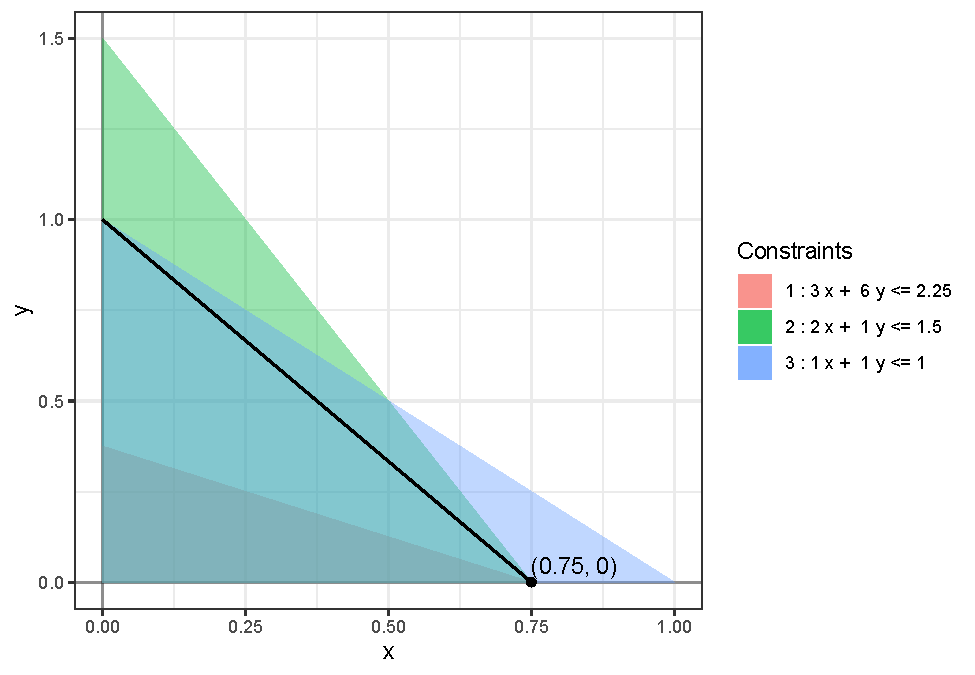
\includegraphics{Introduction-to-Optimization_files/figure-latex/fig-bounds-b1-1.pdf} 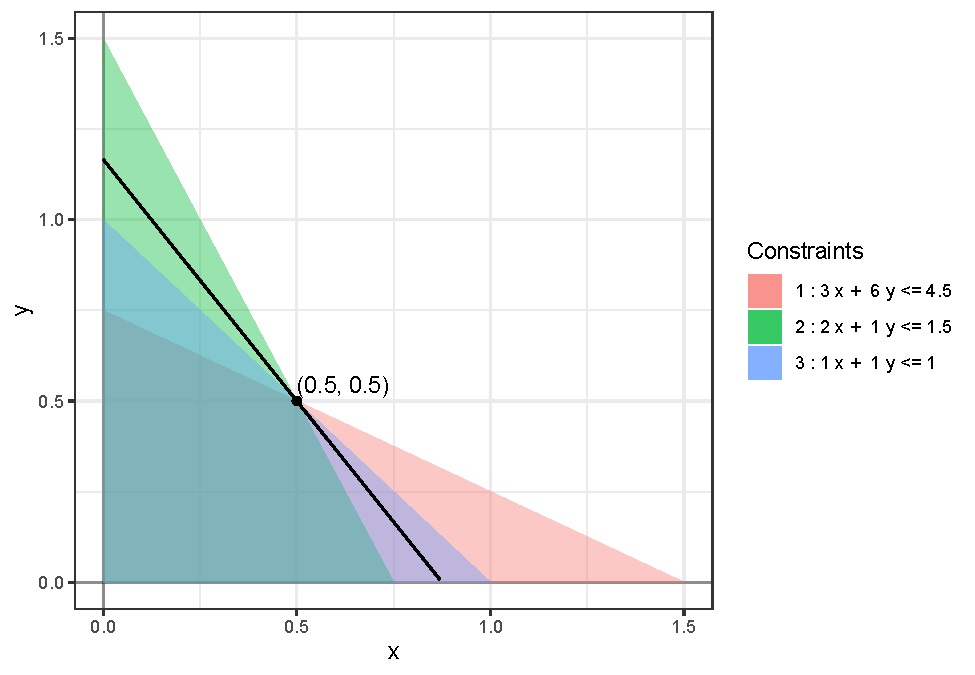
\includegraphics{Introduction-to-Optimization_files/figure-latex/fig-bounds-b1-2.pdf}
\end{example}

\hypertarget{shadow-prices}{%
\section{Shadow Prices}\label{shadow-prices}}

Assume now that neither of \(\delta_+\) or \(\delta_-\) is zero. We can use Lemma \ref{lem:basic-values} to find the rate of change of the optimal solution with respect to \(b_i\). Call the objective function \(\mathbb{O} = c^{T} x\). We think of \(\mathbb{O}\) as being a function of \(b_i\), \(c_j\), and \(a_{ij}.\) Using Lemma \ref{lem:basic-values} we get
\begin{align*}
  \dfrac{\partial x_{\mathcal{B}_j}}{\partial b_i} 
    &= j^{th} \mbox{ row of } \dfrac{\partial \mathcal{B}^{-1}b}{\partial b_i} \\
    &= (\mathcal{B}^{-1})_{ji} \\
\end{align*}
where \(x_{\mathcal{B}_j}\) denotes the \(j^{th}\) basic variable at the optimal solution. And
\begin{align*}
  \dfrac{\partial x_{\mathcal{N}}}{\partial b_i} 
    &= 0
\end{align*}
as the non-basic variables remain 0 when we perturb \(b_i\) within the range of optimality.
Using these we can find the rate of change of the optimal solution \(\mathbb{O}\) with respect to \(b_i\). We first start by re-indexing the variables and objective coefficients using the basic and non-basic variables.
\begin{align*}
  \mathbb{O} 
    &= c^T x \\
    &= c^T_{\mathcal{B}} x_{\mathcal{B}} + c^T_{\mathcal{N}} x_{\mathcal{N}} \\
\implies
  \dfrac{\partial \mathbb{O}}{\partial b_i} 
    &= c^T_{\mathcal{B}} \dfrac{\partial x_{\mathcal{B}}}{\partial b_i} + c^T_{\mathcal{N}} \dfrac{\partial x_{\mathcal{N}}}{\partial b_i} \\
    &= c^T_{\mathcal{B}} (\mathcal{B}^{-1})_{\_i}
\end{align*}
By strong duality, we know that the primal objective value equals the dual objective value i.e.~
\begin{align*}
 \mathbb{O} &= b_1 y_1 + \cdots + b_m y_m 
\end{align*}
So, \(\partial \mathbb{O}/\partial b_i = y_i\). Because of this result, \(y_i\) is also called the \textbf{shadow price} or the \textbf{marginal cost} of the \(i^{th}\) constraint.
Using the rate of change calculation above, we get \begin{align*}
  y_i = c^T_{\mathcal{B}} (\mathcal{B}^{-1})_{\_i}.
\end{align*}
We can combine all the above coordinates into a single vector to get the following result.

\begin{theorem}
\protect\hypertarget{thm:dual-solution}{}\label{thm:dual-solution}For a non-degenerate linear program, the dual optimal solution is given by \((\mathcal{B}^{-1})^Tc_{\mathcal{B}}\).
\end{theorem}

This theorem provides yet another method of finding the dual optimal solution without having to solve the dual linear program.

\begin{example}
\protect\hypertarget{exm:dual-solution}{}\label{exm:dual-solution}For the linear program \eqref{eq:bond-portfolio-lp}, the objective function is
\begin{align*}
  \mathbb{O} & = 4 x + 3y \\
  & = 4x + 3y + 0 w_3 + 0 w_1 + 0 w_2 
\end{align*}

So, \(c_{\mathcal{B}} = \begin{bmatrix}4 \\ 3 \\ 0 \end{bmatrix}\) and \(c_{\mathcal{N}} = \begin{bmatrix}0 \\ 0 \end{bmatrix}\).
Using the value of \(\mathcal{B}^{-1}\) calculated above, we get
\begin{align*}
  y & = (\mathcal{B}^{-1})^Tc_{\mathcal{B}} \\
  & = 
    \begin{bmatrix}
    -1/9 & 2/9 & -1/9 \\
    2/3 & -1/3 & -1/3 \\
    0 & 0 & 1
    \end{bmatrix} 
    \begin{bmatrix}
      4 \\ 3 \\ 0
    \end{bmatrix}\\
  & = 
  \begin{bmatrix}
    2/9 \\ 5/3 \\ 0
  \end{bmatrix}.
\end{align*}
To check that this is indeed dual-optimal, we calculate the dual-objective value at this solution
\begin{align*}
  b^T y & = 3.6 (2/9) + 1.5 (5/3) + 0 (1) \\
  &= 3.3
\end{align*}
which equals the optimal objective value of the primal. One can check that this solution is also dual-feasible and hence is the dual-optimal solution by Certificate of Optimality (Theorem \ref{thm:certificate-of-optimality}).
\end{example}

\hypertarget{sensitivity-analysis---objective}{%
\section{Sensitivity analysis - Objective}\label{sensitivity-analysis---objective}}

We can ask the same questions about the change in the objective coefficients - how far can we change the objective coefficient \(c_j\) without changing the set of basic and non-basic variables at the optimal solution. Note that in this case we are not changing the constraints and therefore the feasible region. So, this is the same as asking - how far can we change the objective coefficient \(c_j\) without changing the optimal solution.

We can redo the entire analysis for the objective coefficients from scratch. However, we can also notice that performing sensitivity analysis on the objective coefficients of the primal is the same as performing sensitivity analysis on the constraints of the dual.
Consider the standardized dual
\begin{equation*}
  \begin{array}{lrll}
    \mbox{maximize: } & -c_0 -b^T y \\
    \mbox{subject to: } 
      & -A^T y & \leq & -c \\
      & y & \geq & 0,
  \end{array}
\end{equation*}
Using Equation \eqref{eq:range-of-optimality} for this dictionary we get the range of optimality for \(-c_j\) to be
\begin{equation}
  (-\mathcal{B}_d)^{-1} (-c) + \delta (-\mathcal{B}_d^{-1})_{\_j} \ge 0.
\end{equation}
where \(-\mathcal{B}_d\) is formed by combining the dual-basic columns of \(\begin{bmatrix} -A^T & I_n\end{bmatrix}\) and so \(\mathcal{B}_d\) is formed by combining the dual-basic columns of \(\begin{bmatrix} A^T & -I_n\end{bmatrix}\). This simplifies to
\begin{equation}
  \mathcal{B}_d^{-1} c - \delta (\mathcal{B}_d^{-1})_{\_j} \ge 0.
\end{equation}
Note that this is the range of optimality for \(-c_j\). To get the range of optimality for \(c_j\) we need to replace \(\delta\) by \(-\delta\) to get
\begin{equation}
  \mathcal{B}_d^{-1} c + \delta (\mathcal{B}_d^{-1})_{\_j} \ge 0.
\end{equation}

Finally, by Lemma \ref{lem:basic-values}, \(\mathcal{B}_d^{-1} c\) is the vector of values of the dual basic variables. Hence we get,

\begin{proposition}
The \textbf{range of optimality} for \(c_j\) is the interval \([c_j + \delta_-, c_j + \delta_+]\) such that \(y_{\mathcal{B}}^* + \delta (\mathcal{B}_d^{-1})_{\_j} \ge 0\) for all \(\delta \in [\delta_-, \delta_+]\).
\end{proposition}

By a happy accident all the negative signs have cancelled out and the equation for finding the range of optimality for the objective coefficients is exactly the same as the one for finding the range of optimality for the constraints.

\begin{theorem}
\protect\hypertarget{thm:range-of-optimality}{}\label{thm:range-of-optimality}The range of optimality for the constraints and the objective functions can be computed using the following formulae:

\textbf{Range of optimality for \(b_i\):}
\begin{equation}
  x_{\mathcal{B}}^* + \delta (\mathcal{B}^{-1})_{\_i} \ge 0.
\end{equation}
where \(\mathcal{B}\) is formed by combining the primal-basic columns of \(\begin{bmatrix} A & I_m \end{bmatrix}\), and

\textbf{Range of optimality for \(c_j\):}
\begin{equation}
  y_{\mathcal{B}}^* + \delta (\mathcal{B}_d^{-1})_{\_j} \ge 0.
\end{equation}
where \(\mathcal{B}_d\) is formed by combining the dual-basic columns of \(\begin{bmatrix} A^T & -I_n \end{bmatrix}\).
\end{theorem}

Finally, to find \(\mathcal{B}_d\) we note that by Complementary Slackness (Theorem \ref{thm:complementary-slackness}), if the linear program is non-degenerate then the dual basic variables correspond to the primal non-basic variables (as the dual basic variables must be non-zero). This statement is true even for degenerate linear programs but in this case the proof is more subtle and requires the use of Strong duality (Theorem \ref{thm:strong-duality}).

\begin{example}
Consider the linear program \eqref{eq:bond-portfolio-lp} again. At the optimal solution, as \(w_1\) and \(w_2\) are non-basic, the corresponding dual variables (\(y_1\) and \(y_2\)) will be basic for the dual linear program \eqref{eq:bond-portfolio-dual}. This gives us
\begin{align*}
  \mathcal{B}_d &= \begin{bmatrix} 3 & 2 \\ 6 & 1 \end{bmatrix} \\
  \implies 
  \mathcal{B}_d^{-1} &= \begin{bmatrix} -1/9 & 2/9 \\ 2/3 & -1/3 \end{bmatrix}.
\end{align*}

From Example \ref{exm:dual-solution} we know that \(y_1 = 2/9\) and \(y_2 = 5/3\) at the dual optimal solution. Using these, we can now find the range of optimality for the objective coefficients.

To find the range of optimality for \(c_1 = 4\) we solve
\begin{align*}
  \begin{bmatrix} 2/9 \\ 5/3 \end{bmatrix} 
  + 
  \delta \begin{bmatrix} -1/9 \\ 2/3 \end{bmatrix} \ge 0
\end{align*}
which gives us the inequalities
\begin{align*}
  \begin{array}{lrlrrll}
  2/9 + \delta (-1/9) & \ge & 0 & \implies & \delta & \le & 2 \\
  5/3 + \delta (2/3) & \ge & 0 & \implies & \delta & \ge & -5/2
  \end{array}
\end{align*}
So, \(\delta_- = -5/2\) and \(\delta_+ = 2\) and the range of optimality for \(c_1\) is \([4 - 5/2, 4 + 2] = [1.5, 6]\).

To find the range of optimality for \(c_2 = 3\) we solve
\begin{align*}
  \begin{bmatrix} 2/9 \\ 5/3 \end{bmatrix} 
  + 
  \delta \begin{bmatrix} 2/9 \\ -1/3 \end{bmatrix} \ge 0
\end{align*}
which gives us the inequalities
\begin{align*}
  \begin{array}{lrlrrll}
  2/9 + \delta (2/9) & \ge & 0 & \implies & \delta & \ge & -1 \\
  5/3 + \delta (-1/3) & \ge & 0 & \implies & \delta & \le & 5
  \end{array}
\end{align*}
So, \(\delta_- = -1\) and \(\delta_+ = 5\) and the range of optimality for \(c_2\) is \([3 - 1, 3 + 5] = [2, 8]\).

The following figures show the (infinitely many) optimal solutions at the extreme ends of the range of optimality of \(c_1\).

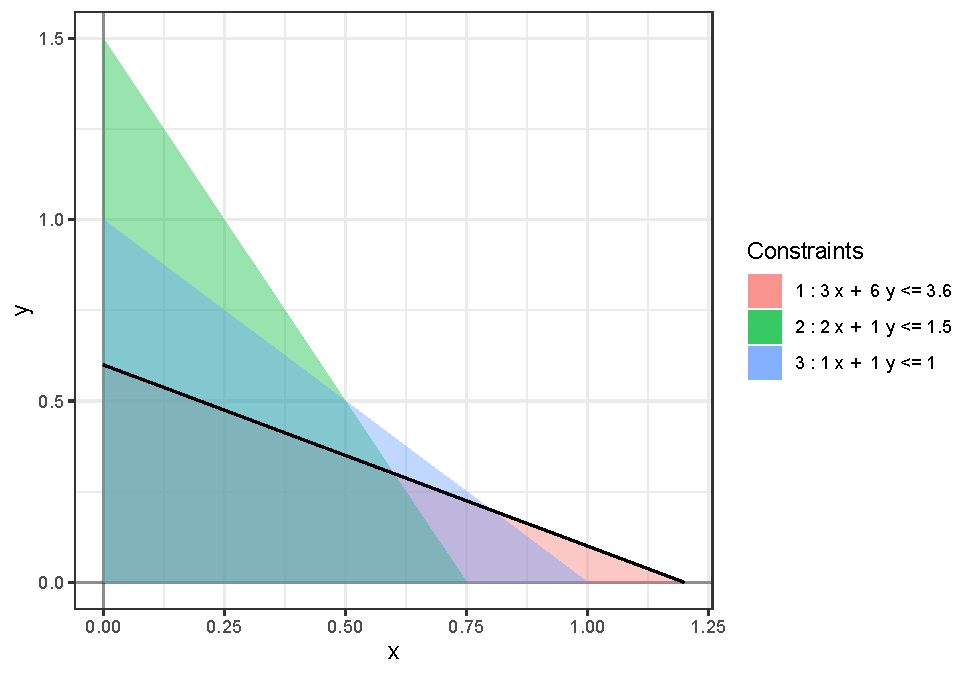
\includegraphics{Introduction-to-Optimization_files/figure-latex/fig-bounds-c1-1.pdf} 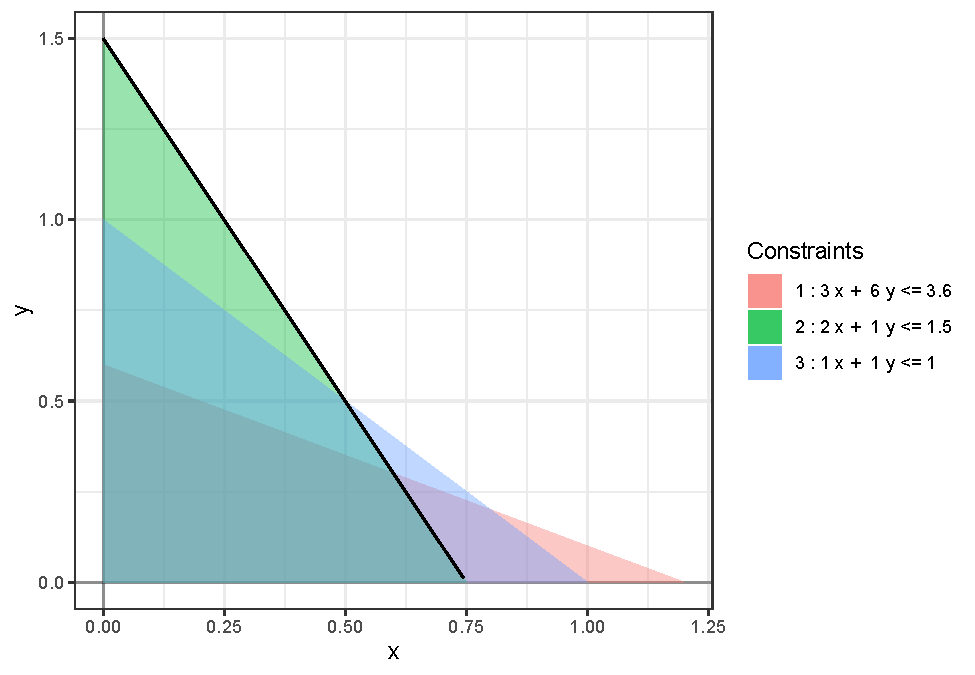
\includegraphics{Introduction-to-Optimization_files/figure-latex/fig-bounds-c1-2.pdf}
\end{example}

\hypertarget{part-non-linear-programming}{%
\part{Non-Linear Programming}\label{part-non-linear-programming}}

\hypertarget{convex-programming}{%
\chapter{Convex Programming}\label{convex-programming}}

We will now move toward generalizing the concepts from linear programming to non-linear optimization questions.
We'll only touch several subjects briefly without going into too much depth.
We'll start with convex optimization, which is a direct generalization of linear programming.

\begin{definition}
We say that a subset \(\mathcal{S}\) of \(\mathbb{R}^n\) is called \textbf{convex} if for any points \({x}_1\) and \({x}_2\) in \(\mathcal{S}\), the line segment connecting them also lies in \(\mathcal{S}\). More precisely, we say that \(S\) is \textbf{convex} if forall \({x}_1\) in \(\mathcal{S}\), \({x}_2\) in \(\mathcal{S}\), and \(t \in [0,1]\), the point \((1 - t) {x}_1 + t {x}_2\) also lies in \(\mathcal{S}\).
\end{definition}

\begin{exercise}
Show that the feasible region of a linear program is convex.
\end{exercise}

\begin{definition}
We say that function \(f : \mathcal{S} \to \mathbb{R}\) is \textbf{convex} if for all \({x}_1\) in \(\mathcal{S}\), \({x}_2\) in \(\mathcal{S}\), and \(t \in [0,1]\), the inequality \(f((1 - t) {x}_1 + t {x}_2) \le (1 - t) f({x}_1) + t f({x}_2)\) holds. Geometrically, this is saying that any line segment connecting two points on the graph of \(f\) lies above the graph.
\end{definition}

The following theorem provides a quick way to check if a function is convex and to come up with examples of convex functions.

\begin{theorem}
\protect\hypertarget{thm:convexity-second-derivative}{}\label{thm:convexity-second-derivative}Let \(f : \mathbb{R}^n \to \mathbb{R}\) be a \(C^2\) function. \(f\) is convex if and only if the Hessian matrix of \(f\) is positive semi-definite. In particular, when \(n = 1\), \(f\) is convex if and only if \(f'' \ge 0\).
\end{theorem}

\begin{definition}
An optimization problem
\begin{equation}
  \begin{array}{ll}
    \mbox{maximize: } & f(x)  \\ 
    \mbox{subject to: } & x \in \mathcal{S} 
  \end{array}
  \label{eq:convex-optimization-problem}
\end{equation}
is called \textbf{convex} if \(\mathcal{S}\) is a closed and convex subset of \(\mathbb{R}^n\) and \(f : \mathcal{S} \to \mathbb{R}\) is a convex function.
\end{definition}

\begin{exercise}
Show that a linear program is a convex optimization problem.
\end{exercise}

The following theorem is an example of how theorems about linear programs generalize to convex programs.

\begin{theorem}
\protect\hypertarget{thm:optimal-on-boundary}{}\label{thm:optimal-on-boundary}The convex optimization problem \eqref{eq:convex-optimization-problem} either has an optimal solution on the boundary of \(\mathcal{S}\) or is unbounded.
\end{theorem}

\begin{proof}
Let \({x}\) be a point in the interior of \(\mathcal{S}\).
It suffices to show that either there is some point on the boundary of \(\mathcal{S}\) with an objective value that is greater than or equal to the objective value of \({x}\) or the problem is unbounded.

Let \({x}_1\) be any point on the boundary of \(\mathcal{S}\). Draw a ray starting at \({x}_1\) in the direction of \({x}\).
As \(\mathcal{S}\) is closed and convex, two cases are possible:

\begin{enumerate}
\def\labelenumi{\arabic{enumi}.}
\tightlist
\item
  The ray intersects the boundary of \(\mathcal{S}\) in exactly one more point, say \({x}_2\).
\item
  The ray does not intersect the boundary of \(\mathcal{S}\) and the entire ray is contained within \(\mathcal{S}\).
\end{enumerate}

\textbf{Case 1:}

We will show that either \(f({x}) \le f({x}_1)\) or \(f({x}) \le f({x}_2)\).
We prove this by contradiction. Suppose \(f({x}) > f({x}_1)\) and \(f({x}) > f({x}_2)\).
We know that \(x = (1 - t) x_1 + t x_2\) for some \(t \in (0, 1)\).
Multiplying the first inequality by \((1-t)\) and the second by \(t\) and adding them together, we get
\begin{align*}
  && (1-t) f({x}) + t f({x}) &> (1-t) f({x}_1) + t f({x}_2) \\ 
  \implies 
  && f({x}) &> (1-t) f({x}_1) + t f({x}_2) ,
\end{align*}
which contradicts the convexity of \(f\).

\textbf{Case 2:}

If \(f(x_1) \ge f(x)\), we're done. Suppose this is not the case. We'll show that the problem is unbounded.

For \(0 < t \le 1\), let \({y}_t\) denote the point on the ray such that
\begin{align*}
  {x} = (1-t) {x}_1 + t {y}_t.
\end{align*}

For example, \({y}_1 = {x}\) and \({y}_{1/2}\) is the point on the ray for which \({x}\) is midpoint of \({x}_1\) and \({y}_{1/2}\). As \(t\) decreases, \({y}_t\) will move farther and farther away from \({x}\). Note that all of \({y}_t\) lie inside \(\mathcal{S}\). By convexity of \(f\), we know that
\begin{align*}
  && f({x}) & \le (1-t) f({x}_1) + t f({y}_  t) \\
\implies && f({x}) - (1-t) f({x}_1) &\le t f({y}_t) \\
\implies && t^{-1}f({x}) - (t^{-1}-1) f({x}_1) &\le f({y}_t) \\
\implies && t^{-1}(f({x}) - f({x}_1)) + f({x}_1) &\le f({y}_t) \\
\end{align*}
As \(f({x}) > f({x}_1)\), the left hand side tends to \(\infty\) as \(t\) decreases and the optimization problem is unbounded.
\end{proof}

The following corollary follows by applying \href{https://en.wikipedia.org/wiki/Extreme_value_theorem}{Extreme Value Theorem} to the above result.

\begin{theorem}
If \(\mathcal{S}\) is bounded (in addition to being closed and convex), then the convex optimization problem \eqref{eq:convex-optimization-problem} has an optimal solution on the boundary of \(\mathcal{S}\).
\end{theorem}

\hypertarget{separation-theorems}{%
\chapter{Separation Theorems}\label{separation-theorems}}

We'll next prove a couple of \emph{geometric} results that are equivalent to strong duality theorem (Theorem \ref{thm:strong-duality}).

\hypertarget{farkas-lemma}{%
\section{Farkas' Lemma}\label{farkas-lemma}}

\begin{theorem}[Farkas' lemma]
\protect\hypertarget{thm:farkas-lemma}{}\label{thm:farkas-lemma}Let \(A\) be an \(m \times n\) matrix and \(b\) be a vector in \(\mathbb{R}^m\).
Exactly one of the following systems has a solution:
\begin{align}
  A x & = b \\ 
  x & \ge 0.
\label{eq:farkas-eq1}
\end{align}
\begin{align}
  y^T A & \ge 0 \\ 
  y^T b & < 0.
\label{eq:farkas-eq2}
\end{align}
\end{theorem}

\begin{proof}
We'll prove Farkas' lemma using strong duality. Consider the following linear program:
\begin{equation}
  \begin{array}{llll}
    \mbox{maximize: } & 0 \\
    \mbox{subject to: } 
      & A x & = & b \\ 
      & x & \ge & 0.
  \end{array}
\label{eq:farkas-primal}
\end{equation}
The optimal solution to the linear program \eqref{eq:farkas-primal} is a feasible solution to \eqref{eq:farkas-eq1}. The dual to this linear program is
\begin{equation}
  \begin{array}{llll}
    \mbox{minimize: } & y^T b \\
    \mbox{subject to: } 
      & y^T A & \ge & 0.
  \end{array}
\label{eq:farkas-dual}
\end{equation}

\textbf{Case 1:} Suppose \eqref{eq:farkas-eq1} has a solution.

In this case, \eqref{eq:farkas-primal} has an optimal solution. By strong duality, \eqref{eq:farkas-dual} also has an optimal solution with optimal objective \(0\). So, the minimum value of \(y^T b\) is \(0\) and hence the system \eqref{eq:farkas-eq2} does not have a solution.

\textbf{Case 2:} Suppose \eqref{eq:farkas-eq1} does not have a solution.

In this case, \eqref{eq:farkas-primal} has no optimal solution. By strong duality, neither does \eqref{eq:farkas-dual}. So, \eqref{eq:farkas-dual} is either infeasible or unbounded. As \(y = 0\) is a feasible solution to \eqref{eq:farkas-dual} it cannot be infeasible, and hence it must be unbounded. But this means that the value of \(y^T b\) can be made arbitrarily small, and in particular, can be made negative. Hence, the system \eqref{eq:farkas-eq2} has a solution.
\end{proof}

We can interpret Farkas' lemma geometrically using convex cones and separating hyperplanes.

\hypertarget{separating-hyperplane-theorem}{%
\section{Separating Hyperplane Theorem}\label{separating-hyperplane-theorem}}

\begin{definition}
The \textbf{convex cone} of a finite set of vectors in \(\mathbb{R}^m\) is the set of positive linear combinations of vectors in the set.\footnote{One can also define convex cones for infinite sets of vectors. In this case, we need to take the closure of the set of positive linear combinations.}
\begin{align*}
  C_+(v_1, \dots, v_n) & := \{c_1 v_1 + \dots + c_n v_n \mid c_i \ge 0 \}.
\end{align*}
\end{definition}

\begin{definition}
A \textbf{hyperplane} in \(\mathbb{R}^m\) is the set of solutions to a single linear equation.
The complement of a hyperplane in \(\mathbb{R}^n\) consists of two connected components.
The closures of these components are called \textbf{half-spaces}.
\end{definition}

If the equation of the hyperplane is given by \(b^T y = b_0\), where \(b\) is a vector in \(\mathbb{R}^m\) and \(b_0 \in \mathbb{R}\), then the corresponding two half-spaces are described by \(b^T y \le b_0\) and \(b^T y \ge b_0\).

\begin{definition}
We say that a hyperplane \(H\) \textbf{separates} two subsets \(S_1\) and \(S_2\) of \(\mathbb{R}^m\) if \(S_1\) and \(S_2\) do not intersect \(H\) and belong to the two different half-spaces of \(H\).
\end{definition}

Using convex cones and separating hyperplanes, we can reinterpret \ref{thm:farkas-lemma} as follows.

\begin{theorem}[Geometric version of Farkas' lemma]
\protect\hypertarget{thm:farkas-geometry}{}\label{thm:farkas-geometry}

Let \(v_1, \dots, v_n, b\) be vectors in \(\mathbb{R}^m\). Exactly one of the following statements is true:

\begin{enumerate}
\def\labelenumi{\arabic{enumi}.}
\tightlist
\item
  Either \(b\) lies inside \(C_+(v_1, \dots, v_n)\), or
\item
  There is a hyperplane \(H\) that separates \(b\) from \(C_+(v_1, \dots, v_n)\).
\end{enumerate}

\end{theorem}

A point \(b\) and a convex cone \(C_+(v_1, \dots, v_n)\) are convex subsets of \(\mathbb{R}^m\).
The statement of Farkas' lemma \ref{thm:farkas-geometry} can be generalized to arbitrary convex sets using metric topology.
For now, we'll generalize it to convex polyhedra.

\begin{definition}
Intersection of finitely many half-spaces is called a \textbf{convex polyhedron}.
\end{definition}

So, a convex polyhedron is the set of solutions to a system of linear inequalities \(A x \le b\).
But this set is precisely the feasible region of a linear program!
The class of convex polyhedra is very large and all geometric ``linear'' convex objects, like points, lines, planes, half-spaces, hyperplanes, convex cones, etc. can be realized as convex polyhedra.

The following is an extension of Farkas' lemma to convex polyhedra (proof in the exercises below).

\begin{theorem}[Separating Hyperplane Theorem]
\protect\hypertarget{thm:separating-hyperplane}{}\label{thm:separating-hyperplane}Any two non-empty, disjoint, convex polyhedra in \(\mathbb{R}^m\) can be separated by a hyperplane.
\end{theorem}

\begin{exercise}
\protect\hypertarget{exr:farkas-variant}{}\label{exr:farkas-variant}

Prove the following variant of Farkas' lemma: Let \(A\) be an \(m \times n\) matrix and let \(b\) be a vector in \(\mathbb{R}^m\).
Exactly one of the following systems has a solution:

\begin{enumerate}
\def\labelenumi{\arabic{enumi}.}
\tightlist
\item
  \(Ax \le b\),
\item
  \(y^T b < 0\), \(y^T A = 0\), and \(y \ge 0\).
\end{enumerate}

\end{exercise}

\begin{exercise}

Let \(P_1\) be the convex polyhedron defined by \(A_1 x \le b_1\) and let \(P_2\) be the convex polyhedron defined by \(A_2 x \le b_2\) where \(A_1\), \(A_2\), \(b_1\), and \(b_2\) have sizes \(m_1 \times n\), \(m_2 \times n\), \(m_1\), and \(m_2\), respectively. Suppose the system
\begin{equation}
  \begin{bmatrix} A_1 \\ A_2 \end{bmatrix}
  x 
  \le
  \begin{bmatrix} b_1 \\ b_2 \end{bmatrix}
  \label{eq:eq1}
\end{equation}
does not have a solution.

\begin{enumerate}
\def\labelenumi{\arabic{enumi}.}
\tightlist
\item
  Apply the above variant of Farkas' lemma to \eqref{eq:eq1} to obtain vectors \(y_1\), \(y_2\) of size \(m_1\) and \(m_2\), respectively. Define \(c^T := y_1^T A_1\), \(d_1 := y_1^T b_1\), and \(d_2 := -y_2^T b_2\).
\item
  Show that \(d_1 < d_2\).
\item
  Show that \(A_1 x \le b_1\) implies \(c^T x \le d_1\).
\item
  Show that \(A_2 x \le b_2\) implies \(c^T x \ge d_2\).
\item
  Conclude that there exists a hyperplane separating \(P_1\) and \(P_2\).
\end{enumerate}

\end{exercise}

\hypertarget{equivalence-with-strong-duality}{%
\section{Equivalence with Strong Duality}\label{equivalence-with-strong-duality}}

It is possible to prove Strong Duality using Farkas' lemma, which itself can be proven using metric topology. So, Strong Duality, Farkas' lemma, and Separating Hyperplane Theorem should all be thought of as equivalent to each other. We provide below a proof of Strong Duality (Theorem \ref{thm:strong-duality}) using Farkas' lemma.

\begin{proof}
Consider the system of equations

\begin{equation}
\begin{split}
Ax & \le b \\
-A^T y & \le -c \\ 
x, y & \ge 0 \\
-c^T x + b^T y & \le 0.
\end{split}
\label{eq:strong-using-farkas}
\end{equation}

Suppose this system has a feasible solution. The first three equations are equivalent to saying that \(x\) is primal-feasible and \(y\) is dual-feasible. If such a solution exists, by Weak Duality (Theorem \ref{thm:weak-duality}) we know that \(c^T x \le b^T y\). So, the only way the fourth inequality is satisfied is if \(c^T x = b^T y\) i.e.~the primal-objective value at \(x\) equals the dual-objective value at \(y\). But by Weak Duality, these must then be the optimal solutions thereby proving Strong Duality. So, it suffices to show that \eqref{eq:strong-using-farkas} has a feasible solution if the primal has an optimal solution.

We prove this by contradiction. Suppose the primal has an optimal solution but \eqref{eq:strong-using-farkas} does not have a feasible solution. We rewrite the system as
\begin{align*}
    \begin{bmatrix} A & 0 \\ 0 & -A^T \\ -c^T & b^T \end{bmatrix}
    \begin{bmatrix} x \\ y  \end{bmatrix}
      & \le 
    \begin{bmatrix} b \\ -c \\ 0 \end{bmatrix} \\
    x, y & \ge 0.
\end{align*}
By (a variant of) Farkas' lemma, the following dual system must have a solution.
\begin{align*}
  \begin{bmatrix} z^T & w^T & t \end{bmatrix}
  \begin{bmatrix} b \\ -c \\ 0 \end{bmatrix} & < 0 \\
  \begin{bmatrix} z^T & w^T & t \end{bmatrix}
    \begin{bmatrix} A & 0 \\ 0 & -A^T \\ -c^T & b^T \end{bmatrix}
    & \ge 0\\
  z, w, t & \ge 0.
\end{align*}
which can be rewritten as
\begin{align*}
    z^T b & < w^T c \\
    z^T A & \ge t c^T \\
    t b^T & \ge w^T A^T \\
    z, w, t & \ge 0.
\end{align*}
By combining the second and third equations, we get
\begin{align*}
    t z^T b \ge z^T A w \ge t c^T w.
\end{align*}
If \(t > 0\), this contradicts the first equation and we're done. So suppose \(t = 0\). Plugging in \(t = 0\), we get
\begin{align*}
    z^T b & < w^T c \\
    z^T A & \ge 0 \\
    0 & \ge w^T A^T \\
    z, w & \ge 0.
\end{align*}
which can be rewritten as the matrix equation
\begin{align*}
  \begin{bmatrix} z^T & w^T \end{bmatrix}
  \begin{bmatrix} b \\ -c \end{bmatrix} & < 0 \\
  \begin{bmatrix} z^T & w^T \end{bmatrix}
    \begin{bmatrix} A & 0 \\ 0 & -A^T \end{bmatrix}
    & \ge 0\\
  z, w & \ge 0.
\end{align*}
Because this system has a solution, by applying (variant of) Farkas' lemma again, the following system cannot have a solution.
\begin{align*}
    \begin{bmatrix} A & 0 \\ 0 & -A^T \end{bmatrix}
    \begin{bmatrix} x \\ y  \end{bmatrix}
      & \le 
    \begin{bmatrix} b \\ -c \end{bmatrix} \\
    x, y & \ge 0.
\end{align*}
We had assumed that the primal is feasible. The only way the above system is infeasible is if there is no solution no the system
\begin{align*}
  A^T y &\ge c \\
  y &\ge 0.
\end{align*}
Applying (variant of) Farkas' lemma yet again we see that the dual system
\begin{align*}
  z^T c & < 0\\
  z^T A^T &\ge 0 \\ 
  z &\le 0
\end{align*}
must have a solution.
But now, if \(x\) is any primal-feasible solution then so is \(x - \alpha z\) for any positive constant \(\alpha\) and the objective value of the primal at \(x - \alpha z\) can be made arbitrarily large by increasing \(\alpha\) thereby contradicting the fact that primal has an optimal solution (and hence is bounded).
\end{proof}

\hypertarget{interior-point-method}{%
\chapter{Interior Point Method}\label{interior-point-method}}

Throughout this chapter we will let \(f\) denote a twice differentiable function from \(\mathbb{R}^n\) to \(\mathbb{R}\).

\hypertarget{gradient-descent}{%
\section{Gradient Descent}\label{gradient-descent}}

We will start by trying to solve the following unconstrained optimization problem:
\begin{align*}
  \mbox{minimize: } & f(x)
\end{align*}
where \(x\) is any vector in \(\mathbb{R}^n\).
\textbf{Gradient descent} is a simple algorithm for solving this problem using basic differential calculus.
It relies on the fact that \emph{the negative of the gradient points in the direction in which the function decreases the fastest}.
So the general principle is to move in the direction of the negative gradient until the function is no longer decreasing.
More precisely, we create a sequence of guesses using the following GD recurrence relation:
\[x_{k+1} = x_k - t_k \nabla f(x_k)\]
where \(t_k\) is the ``step size'' for the \(k^{th}\) iteration and can be chosen to be a small constant or some function of \(k\), \(x_k\), \(f(x_k)\), or \(\nabla f(x_k)\).

There are several issues with this technique:

\begin{enumerate}
\def\labelenumi{\arabic{enumi}.}
\tightlist
\item
  If the function has multiple local minima, then the sequence might converge to a non-absolute minima depending on the starting guess and the choice of step sizes.
\item
  If the step sizes are chosen to be too large, then the sequence can completely miss the minima and may not converge.
\item
  If the step sizes are chosen to be too small, then the sequence may take a long time to converge.
\end{enumerate}

Unfortunately, there is no easy way to resolve these issues. In practice, either we need some additional information about the function and its gradient or we proceed by trial and error to find step sizes that work. Even then there is no guarantee that the algorithm will converge to an absolute minima and not a local minima, if at all. In spite of these issues, because of its simplicity, ease of implementation, and good convergence properties in practice, Gradient Descent is a very popular algorithm for solving unconstrained optimization problems.

\hypertarget{interior-point-method-1}{%
\section{Interior Point Method}\label{interior-point-method-1}}

Gradient descent can be modified to solve constrained optimization problems by introducing barrier functions.
Consider the following problem:
\begin{equation}
  \begin{array}{llr}
    \mbox{minimize: } & f(x) \\
    \mbox{subject to: } & g_i(x) \ge 0, & \mbox{ for } 1 \le i \le m. \\
  \end{array}
  \label{eq:constrained-optimization-problem}
\end{equation}
We can apply GD to this problem and find a critical point for \(f(x)\). However, this might not answer the optimization question for two reasons:

\begin{enumerate}
\def\labelenumi{\arabic{enumi}.}
\tightlist
\item
  The critical point might not be in the feasible region.
\item
  The optimal solution might not be obtained at a critical of \(f(x)\) and could lie on the boundary \(g(x) = 0\) of the feasible region.
\end{enumerate}

Gradient descent algorithm only \emph{sees} the objective function and does not \emph{know} about the constraints. So, we modify the objective function to include the constraints using barrier functions.

\begin{definition}
A \textbf{barrier function} is a differentiable function \(b\) from \((0, \infty)\) to \(\mathbb{R}\) that has the property \(\lim \limits_{x \to 0^+} f(x) = \infty\).
\end{definition}

We'll use the barrier function \(-\ln x\). Using a small positive parameter \(\mu\), we create a new objective function:
\begin{align*}
  f_\mu(x) := & f(x) - \mu \sum \limits_{i = 1} ^ m \ln (g_i(x)).
\end{align*}
Consider the unconstrained optimization problem
\begin{align*}
  \mbox{minimize: } & f_\mu (x).
\end{align*}
Because the domain of \(\ln x\) is \((0, \infty)\), any critical point of \(f_\mu(x)\) must lie in the feasible region of \eqref{eq:constrained-optimization-problem}.
Let \(x_\mu^*\) be a solution of the above problem.
For sufficiently good functions \(f\) and \(g_i\), \emph{\(x_\mu^*\) exists and is continuous in \(\mu\) and \(\lim \limits_{\mu \to 0^+} x_\mu^* = x^*\) where \(x^*\) is an optimal solution to \eqref{eq:constrained-optimization-problem}.} This assumption is valid, for example, for linear programs. With this assumption, we now have a method for solving \eqref{eq:constrained-optimization-problem}:

\begin{itemize}
\tightlist
\item
  Start with a small \(\mu_0 > 0\) and optimize \(f_{\mu_0}(x)\) using GD. Call the solution \(x_{\mu_0}^*\).
\item
  Repeat the following until the sequence \(x_{\mu_k}^*\) stabilizes sufficiently:

  \begin{enumerate}
  \def\labelenumi{\arabic{enumi}.}
  \tightlist
  \item
    Set \(\mu_{k+1} = \mu_k - \delta_k\) for some small \(\delta_k\).
  \item
    Using \(x^*_{\mu_k}\) as a starting point for GD, optimize \(f_{\mu_{k+1}}(x)\). Call the solution \(x_{\mu_{k+1}}^*\).
  \item
    Increase \(k\) to \(k + 1\).
  \end{enumerate}
\end{itemize}

This method is a very simplified \textbf{interior point method}. The sequence of points \(x_{\mu}\) is called the \textbf{central path}.

\begin{example}
\protect\hypertarget{exm:ip-kkt}{}\label{exm:ip-kkt}We can compute the central path explicitly for some simple examples. Consider the optimization problem:
\begin{equation}
  \begin{split}
  \mbox{minimize: } & (x + 1)^2 \\
  \mbox{subject to: } & x \ge 0.
  \end{split}
  \label{eq:ip}
\end{equation}
We can calculate the central path as follows:
\begin{align*}
  f_\mu(x) := (x + 1)^2 - \mu \ln (x).
\end{align*}
The critical points for this function can be obtained by setting the derivative to 0.
\begin{align*}
  f'_\mu(x) &= 0 \\ 
  \implies 2(x + 1) - \dfrac{\mu}{x} &= 0 \\
  \implies x^2 + x - \mu/2 &= 0 \\
  \implies x &= \dfrac{-1 \pm \sqrt{1 + 2 \mu}}{2}.
\end{align*}
Only one of the two satisfy \(x \ge 0\), so we get
\begin{align*}
  x_\mu^* = \dfrac{-1 + \sqrt{1 + 2 \mu}}{2}. 
\end{align*}
This is the central path. Taking the limit as \(\mu \to 0\) we get,
\begin{align*}
  \lim \limits_{\mu \to 0^+} x_\mu^* 
  & = \lim \limits_{\mu \to 0^+} \dfrac{-1 + \sqrt{1 + 2 \mu}}{2} \\ 
  &= 0,
\end{align*}
which is indeed the optimal solution for the optimization problem \eqref{eq:ip}.
\end{example}

\hypertarget{kkt-conditions}{%
\chapter{KKT conditions}\label{kkt-conditions}}

We can use the central path to derive some conditions for optimality.
Consider the optimization problem \eqref{eq:constrained-optimization-problem} again.
As before, we'll assume that \emph{there is a central path \(x_\mu^*\) converging to an optimal solution \(x^*\).}
Because \(x_\mu^*\) is a critical point of \(f_\mu(x)\), we get
\begin{align*}
  \nabla_x f_\mu(x_\mu^*) &= 0 \\
  \implies \nabla f(x_\mu^*) - \sum \limits_{i = 1}^m \dfrac{\mu}{g_i(x_\mu^*)} \nabla g_i (x_\mu^*)&= 0 
\end{align*}
Applying \(\lim \limits_{\mu \to 0^+}\) to both sides, we get
\begin{align*}
   \lim \limits_{\mu \to 0^+} \nabla f(x_\mu^*) - \sum \limits_{i = 1}^m \lim \limits_{\mu \to 0^+}\dfrac{\mu}{g_i(x_\mu^*)} \nabla g_i (x_\mu^*)&= 0 
\end{align*}
which simplifies to
\begin{align*}
  \nabla f(x^*) = \sum \limits_{i = 1}^m \lambda_i \nabla g_i (x^*) 
\end{align*}
where \(\lambda_i = \lim \limits_{\mu \to 0^+}\frac{\mu}{g_i(x_\mu^*)}\) for \(1 \le i \le m\). (There are several assumptions here about the existence and convergence of limits that we're brushing under the rug.)
We can further analyze the constants \(\lambda_i\).
\begin{align*}
  && \dfrac{\mu}{g_i(x_\mu^*)} \cdot g_i(x_\mu^*) &= \mu \\ 
  \implies && \lim \limits_{\mu \to 0^+}\dfrac{\mu}{g_i(x_\mu^*)} \cdot \lim \limits_{\mu \to 0^+}g_i(x_\mu^*) &= \lim \limits_{\mu \to 0^+}\mu \\ 
  \implies &&\lambda_i g_i(x^*) &= 0.
\end{align*}
Finally, because \(g_i(x_\mu^*) \ge 0\) and \(\mu > 0\), we must have
\begin{align*}
  \lambda_i \ge 0.
\end{align*}
To summarize, if \(x^*\) is an optimal solution to \eqref{eq:constrained-optimization-problem} and there exists a central path \(x_\mu^*\) converging to \(x^*\), then the following conditions are satisfied:
\begin{align*}
  \nabla f(x^*) &= \sum \limits_{i = 1}^m \lambda_i \nabla g_i (x^*) \\
  \lambda_i g_i(x^*) &= 0 \\
  \lambda_i &\ge 0.
\end{align*}
These are called the KKT conditions.
We can combine the above derivation with Lagrange multipliers to get the following generalization:

\begin{theorem}[KKT conditions]
\protect\hypertarget{thm:kkt-conditions}{}\label{thm:kkt-conditions}Consider the optimization problem:
\begin{equation*}
  \begin{array}{llr}
    \mbox{minimize: } & f(x) \\
    \mbox{subject to: } 
      & g_i(x) \ge 0, & \mbox{ for } 1 \le i \le m \\
      & h_i(x) = 0, & \mbox{ for } 1 \le i \le k.
  \end{array}
\end{equation*}
Assume that this problem has an optimal solution \(x^*\) and there is a central path \(x_\mu^*\) converging to \(x^*\).
Then under certain regularity conditions, the following conditions are satisfied:
\begin{align*}
  \nabla f(x^*) &= \sum \limits_{i = 1}^m \lambda_i \nabla g_i (x^*) 
  + \sum \limits_{i = 1}^k \lambda'_i \nabla h_i (x^*) \\
  \lambda_i g_i(x^*) &= 0, \mbox{ for } 1 \le i \le m \\
  \lambda_i &\ge 0, \mbox{ for } 1 \le i \le m.
\end{align*}
\end{theorem}

The conditions for necessity, sufficiency and the regularity conditions are quite non-trivial and are beyond the scope of this course.

\begin{example}
Consider Example \ref{exm:ip-kkt} again. The KKT conditions for this example are
\begin{align*}
  2(x + 1) &= \lambda \\
  \lambda x &= 0 \\
  \lambda &\ge 0.
\end{align*}
These need to be satisfied in addition to the original constraint \(x \ge 0\). The only solution to this system is \(x = 0\), which is indeed the optimal solution.
\end{example}

\begin{example}
Consider the linear program
\begin{align*}
  \mbox{minimize: } & c^T x \\
  \mbox{subject to: } & Ax \ge b 
\end{align*}
The KKT conditions for this problem are
\begin{align*}
  c &= A^T \lambda \\
  x_i \lambda _i &= 0, \mbox{ for } 1 \le i \le n,\\
  \lambda &\ge 0.
\end{align*}
This is precisely the dual of the linear programming problem and \emph{complementary slackness} conditions.
Thus the KKT conditions recover duality in the linear programming sense.
\end{example}

\begin{exercise}
Find the KKT conditions for the standard linear program
\begin{align*}
  \mbox{maximize: } & c^T x \\
  \mbox{subject to: } & Ax \le b \\ 
  & x \ge 0.
\end{align*}
Explain how these conditions recover the dual constraints and complementary slackness.
\end{exercise}

\hypertarget{part-applications}{%
\part{Applications}\label{part-applications}}

\hypertarget{l1-regression}{%
\chapter{L1-Regression}\label{l1-regression}}

Linear regression is a method for modelling the relationship between outputs and inputs using linear functions.
Suppose that the data set consists of the points \((x_i, y_i)\) with \(i = 1, 2, ..., N\) where each \(x_i\) is itself a vector in \(\mathbb{R}^m\).
We want to find a function \(f : \mathbb{R}^m \to \mathbb{R}\) such that \(f(x_{i}) \approx y_{i}\).
In linear regression, we suppose that the function \(f\) is of the form \[f(x) = \beta^T x + \beta_0,\] where \(\beta\) is a vector in \(\mathbb{R}^m\) and \(\beta_0\) is a constant.
Our goal is to estimate \(\beta\) and \(\beta_0\).
There is of course, no reason that there is a linear relation between the inputs \(x_i\) and the outputs \(y_i\).
So our is simply to find the \emph{best} estimate.
We can define the error in estimation to be the vector \(\varepsilon\) whose components are
\begin{align*}
  \varepsilon_i = \lvert y_i - f(x_i) \rvert.
\end{align*}
We wish to ``minimize'' the vector in \(\varepsilon\).
There are multiple measures one can define on the space of these errors and minimizing each provides us a best estimate in the sense of that particular measure.

The most commonly used measure is the Euclidean distance or the \(L^2\)-norm. We define
\begin{align*}
  \| \varepsilon_i \|_2 = \sum \limits_{i = 1}^N (y_i - f(x_i))^2 .
\end{align*}
In \(L^2\)-regression we try to find the function \(f\) that minimizes this quantity.
There are several reasons why this measure is most commonly used, one of which being that there is a closed form for the solution using the \href{https://en.wikipedia.org/wiki/Ordinary_least_squares\#Matrix/vector_formulation}{normal equation}.
However, the solution obtained from \(L^2\)-regression is very susceptible to outliers.
By comparison, the \(L^1\)-measure, defined below, is more robust to outliers.
\begin{align*}
  \| \varepsilon_i \|_1 = \sum \limits_{i = 1}^N \lvert y_i - f(x_i) \rvert.
\end{align*}
The biggest downside of \(L^1\) is that it does not have a closed form solution.
However, it is possible to reduce the problem of finding the best \(L^1\)-estimate to linear programming.

Our goal is to solve the following unconstrained minimization problem
\begin{align*}
  \mbox{minimize:} \sum \limits_{i = 1}^N \lvert y_i - (\beta^T x_i + \beta_0) \rvert,
\end{align*}
where our variables are \(\beta\) and \(\beta_0\).
As stated, this problem is not a linear program.
However, it is equivalent to the following linear program:
\begin{equation*}
  \begin{array}{lllr}
    \mbox{minimize:} & \sum \limits_{i = 1}^N \varepsilon_i \\
    \mbox{subject to:} 
      & y_i - (\beta^T x_i + \beta_0) & < & \varepsilon_i \\
      & y_i - (\beta^T x_i + \beta_0) & > & -\varepsilon_i.
  \end{array}
\end{equation*}
Here the decision variables are \(\beta\) (which is a vector in \(\mathbb{R}^m\)), \(\beta_0\), and \(\varepsilon_i\) for \(1 \le i \le N\).

\hypertarget{network-flow}{%
\chapter{Network Flow}\label{network-flow}}

One very important application of linear programming is to finding max-flows in graphs.
The setup is as follows:
we have a simple directed graph \(G = (V, E)\) where \(V\) is the set of vertices and \(E \subseteq V \times V\) is the set of directed edges. Each edge has a non-negative \textbf{capacity} given by a function \(c: E \to \mathbb{R}_{\ge 0}\).
For simplicity, we can assume that capacity is a function \(c : V \times V \to \mathbb{R}_{\ge 0}\) such that \(c(v, v') = 0\) if there is no edge going from \(v\) to \(v'\).
There are two special vertices called \textbf{source} and \textbf{sink} denotes \(s\) and \(t\), respectively.
The source \(s\) has the property that every edge connected to the source points away from it i.e.~there no incoming edges and the sink \(t\) has the property that every edge connected to the sink points toward it i.e.~there no outgoing edges.
Such a graph is called a \textbf{network}.

A \textbf{flow} is a function \(f : E \to \mathbb{R}\) with the property that \(f \le c\). As before, we can assume that \(f\) is a function \(V \times V \to \mathbb{R}\). A flow is said to be balanced if at each vertex the incoming flow equals the outgoing flow. The \textbf{max-flow} question is to find a balanced flow that maximizes the net outflow from the source. More precisely,

\begin{equation*}
\begin{array}{lrllllllllll}
  \mbox{maximize:} & \sum \limits_{v \in V} f(s, v) \\
  \mbox{subject to:} 
  & f(v, w) & \le & c(v, w) & \mbox{ for all } v, w \in V \\
  & \sum \limits_{w \in V} f(v, w) & = & \sum \limits_{w \in V} f(w, v) & \mbox{ for all } v \in V.
\end{array}
\end{equation*}
This is very clearly a linear program that can be solved using the simplex method.
Note however, that several faster algorithms exist for solving this problem.

\hypertarget{min-cut}{%
\section{Min-cut}\label{min-cut}}

The dual of the max-flow problem has an interesting interpretation.
Suppose \(y(v, w)\) are the dual decision variables corresponding to the first kind of constraints and \(z(v)\) are the dual decision variables corresponding to the second kind of constraints.
\begin{equation*}
\begin{array}{lrllllllllll}
  \mbox{minimize:} & \sum \limits_{(v, w) \in V \times W} c(v, w) y(v, w) \\
  \mbox{subject to:} 
  & y(v, w) & \ge & z(v) - z(w) & \mbox{ for all } v, w \in V \\
  & z(s) &= &1 \\
  &z(t) &= &0 \\
  & y(v,w) & \ge & 0 &  \mbox{ for all } v, w \in V. 
\end{array}
\end{equation*}

Consider the graph \(G\) again.
A \textbf{directed path} from the source \(s\) to a sink \(t\) is a sequence of edges of the form \((s, v_1)\), \((v_1, v_2)\), \(\dots\), \((v_{k-1}, v_k)\), \((v_k, t)\) in \(E\).
A subset of edges \(S \subseteq E\) is called an \textbf{s-t cut} if after deleting the edges in \(S\) there is no directed path from \(s\) to \(t\).
Every s-t cut provides a feasible solution to the dual problem as follows: We set \(y(v, w) = 1\) if \((v, w)\) is in the cut, 0 otherwise. We set \(z(v)\) equal 1 if there is a path from \(s\) to \(v\) after making the cut \(S\), 0 otherwise. One can check that the constraints of the dual linear program are indeed satisfied by such a solution.

In fact, a much stronger statement is true. The optimal solution to the dual problem is of this form i.e.~it comes from an s-t cut.
The proof of this statement is beyond the scope of this class.
The \textbf{size} of an s-t cut is the sum of capacities of the edges in the cut.
And thus the dual problem is equivalent to finding a \textbf{min-cut} in the graph \(G\).

\hypertarget{integer-programming}{%
\chapter{Integer Programming}\label{integer-programming}}

An \textbf{integer program} is a linear program in which some or all of the variables are required to be integers. The most common constraint is usually that some variable is required to be either 0 or 1.
Even though integer programs are slight generalizations of linear programs, they are much harder to solve.
It can be shown that solving a general integer program is an NP-hard problem i.e.~we do not expect to there be any efficient algorithm to solve them.
The best we can hope for is to analyze some special kinds of integer programs or to find approximation algorithm for the general case.

One naive approach to solve an integer program is to simply forget the integrality condition and solve the underlying linear program.
This technique is called \textbf{LP-relaxation}.
For nice integer programs, we can expect this method to provide a good approximate solution. However, this method can also provide really incorrect answers.
Consider the following integer program
\begin{equation*}
\begin{array}{lllll}
  \mbox{maximize:} & x \\ 
  \mbox{subject to:} & y & \le & \dfrac{x}{n-0.5} \\
  & x, y & \ge & 0 \\ 
  & x, y & & \mbox{ are integers,}
\end{array}
\end{equation*}
where \(n\) is a fixed integer.
One can check that the feasible region for the LP-relaxation is a triangle with vertices \((0,0)\), \((1,0)\) and \((n - 0.5, 1)\) and the only integer points in this triangle are \((0,0)\) and \((1,0)\).
So, the optimal solution to the LP-relaxation is \((n - 0.5, 1)\) but the optimal solution to the original integer program is \((1,0)\).
Hence, as \(n\) increases the LP solution diverges away from the IP solution.

\hypertarget{branch-and-bound}{%
\section{Branch and Bound}\label{branch-and-bound}}

One technique for fixing the issues with LP-relaxation is called brand-and-bound.
In branch-and-bound we solve the LP-relaxation if we end with a non-integer solution, say with \(x = k\) then we make two cases \(x \le \lfloor k \rfloor\) and \(x \ge \lceil k \rceil\). The goal is to shrink the feasible region so that all the vertices have integer coordinates.
We repeat the process for each case, essentially performing a DFS until we find integer solutions.
This is best demonstrated with an example.

Consider the integer program:
\begin{equation}
\begin{array}{llllll}
  \mbox{maximize:} & 4x & + & 5y \\ 
  \mbox{subject to:} 
  & x & + & y & \le & 10 \\
  & 3x & - & 4y & \le & 6 \\
  & x &, & y & \ge & 0 \\ 
  & x, y & & & & \mbox{ are integers.}
\end{array}
\end{equation}
Solving the LP-relaxation gives us the solution \((x,y) = (4, 1.5)\).
As the \(y\)-coordinates is not an integer, we make two cases \(y \le 1\) and \(y \ge 2\) and analyze each separately by adding it as an extra constraint.
\begin{equation*}
\begin{array}{llllll}
  \mbox{maximize:} & 4x & + & 5y \\ 
  \mbox{subject to:} 
  & x & + & y & \le & 10 \\
  & 3x & - & 4y & \le & 6 \\
  & x &, & y & \ge & 0 \\ 
  & x, y & & & & \mbox{ are integers.} \\
  & & & y & \le & 1 
\end{array}
\end{equation*}
In this case, the optimal solution to the LP-relaxation is \((x,y) = (3.342, 1)\).
This time \(x\) is not an integer, so we make further two cases \(x \le 3\) and \(x \ge 4\).
In the first case, we get
\begin{equation*}
\begin{array}{llllll}
  \mbox{maximize:} & 4x & + & 5y \\ 
  \mbox{subject to:} 
  & x & + & y & \le & 10 \\
  & 3x & - & 4y & \le & 6 \\
  & x &, & y & \ge & 0 \\ 
  & x, y & & & & \mbox{ are integers.} \\
  & & & y & \le & 1 \\
  &x & & & \le & 3,
\end{array}
\end{equation*}
which has the optimal solution \((x,y) = (3, 1)\).
In the second case, we get
\begin{equation*}
\begin{array}{llllll}
  \mbox{maximize:} & 4x & + & 5y \\ 
  \mbox{subject to:} 
  & x & + & y & \le & 10 \\
  & 3x & - & 4y & \le & 6 \\
  & x &, & y & \ge & 0 \\ 
  & x, y & & & & \mbox{ are integers.} \\
  & & & y & \le & 1 \\
  &x & & & \ge & 4,
\end{array}
\end{equation*}
the LP-relaxation and hence the integer program is infeasible.
Going back we are left to analyze the case \(y \ge 2\).
\begin{equation*}
\begin{array}{llllll}
  \mbox{maximize:} & 4x & + & 5y \\ 
  \mbox{subject to:} 
  & x & + & y & \le & 10 \\
  & 3x & - & 4y & \le & 6 \\
  & x &, & y & \ge & 0 \\ 
  & x, y & & & & \mbox{ are integers.} \\
  & & & y & \ge & 2.
\end{array}
\end{equation*}
This has an optimal solution \((x, y) = (2, 2)\).

Thus we have two possible candidates for optimal solutions to the integer program: \((3, 1)\) and \((2, 2)\). We check the objective value \(4x + 3y\) at each of these to conclude that \((2, 2)\) is indeed the optimal solution with objective value 18.

\hypertarget{references}{%
\chapter*{References}\label{references}}


  \bibliography{references.bib}

\printindex
\nocite{*}

\end{document}
